% vim: ts=2 sw=2 et:
\documentclass[xetex]{beamer}
\usetheme{hsr}

\usepackage[T1]{fontenc}
\usepackage{cmbright}
\usepackage{unicode-math}

\usefonttheme{structurebold}

\usepackage{amsmath}
\usepackage{amssymb}

\usepackage{tikz}

\usetikzlibrary{backgrounds}
\usetikzlibrary{bending}
\usetikzlibrary{calc}
\usetikzlibrary{decorations.pathreplacing}
\usetikzlibrary{fadings}
\usetikzlibrary{matrix}
\usetikzlibrary{overlay-beamer-styles}
\usetikzlibrary{positioning}
\usetikzlibrary{trees}

\pgfdeclarelayer{bg}
\pgfsetlayers{bg,main}

\tikzset{
  pics/db/.style args = {#1}{
    code = {
      % FIXME: rewrite using cylinder shapes from shapes library
      \draw[white, fill=white] (-.6,-.7) rectangle (.6,.7);
      \draw[white, fill=white] (0,.7) ellipse [x radius=.6,y radius=.15];
      \foreach \y [count=\i] in {-.7,-.2,.3}
      {
        \draw[thick, fill=white]
          (-0.6,\y) to [looseness=0.5,bend right=90] node[midway] (#1-b-\i) {} ++(1.2,0)
                to node[midway] (#1-e-\i) {} ++(0,0.4)
                to [looseness=0.5,bend left=90] ++(-1.2,0)
                to node[midway] (#1-w-\i) {}++(0,-0.4);
        \draw[thick] (-0.6,\y+0.4) edge[looseness=0.5,bend left=90] node[midway] (#1-t-\i) {} ++(1.2,0);
      }
      \node (#1-north) at (#1-t-3) {};  % [circle,fill=red,minimum size=1mm,inner sep=0pt]
      \node (#1-south) at (#1-b-1) {};  % [circle,fill=red,minimum size=1mm,inner sep=0pt]
      \node (#1-west) at (#1-w-2) {};   % [circle,fill=red,minimum size=1mm,inner sep=0pt]
      \node (#1-east) at (#1-e-2) {};   % [circle,fill=red,minimum size=1mm,inner sep=0pt]
      \node (#1) at ($(#1-north)!0.5!(#1-south)$) {};
    },
  },
  pics/file/.style args = {#1 #2 #3}{
    code = {
      % Rectangle
      \node[
        outer sep = 0, inner sep = 0,
        minimum width = 1cm, minimum height = 1.2cm,
        #3
      ] (#1) {#2};
      % Paper outline
      \draw[thick, fill = white]
        ({#1}.north west) -- ($({#1}.north east) - (.3,0)$)
          -- ++(0,-.3) -- ++(.3,0) -- ({#1}.south east)
          -- ({#1}.south west) -- ({#1}.north west) -- cycle;
      % Fill inside paper
      \draw[fill = white] 
        ($({#1}.north east) - (.3,0)$) to ++(0,-.3) 
        to ++(.3,0) to ++(-.3,.3) to cycle;
      % Paper angle
      \draw[black, thick] ($({#1}.north east) - (.3,0)$) to ++(.3,-.3);
      % Text inside paper
      \node[
        outer sep = 1mm,
        inner sep = 0,
        minimum width = 1cm,
        minimum height = 1.2cm,
      ] (#1) at (#1) {#2};
    },
  },
}

\title{
  Introduction to Git
}
\subtitle{
  ``The stupid\footnote{
    \emph{git} (British) -- a foolish or worthless person}
  content tracker''
}
\author{
  Naoki Pross --- \texttt{np@0hm.ch}
}
\institute{}

\date{11. March 2025}

\AtBeginSection[]
{
  \begin{frame}[shrink]{Table of Contents}
    \tableofcontents[
      currentsection,
      hideothersubsections,
      sectionstyle=show/shaded,
    ]
  \end{frame}
}

\begin{document}

\frame{\titlepage}

\begin{frame}[fragile]{About Me, You and Polls}
  \begin{columns}[b]
    \begin{column}{.5\linewidth}
      \begin{block}<1->{Me}
        \begin{itemize}
          \item BSc in Electrical Engineering OST FH (here)
          \item MSc in EE spec. Control Theory (Regelungstechnik) at ETHZ
          \item For today ``Git connaisseur''
          \item Languages for questions: EN / DE / CH / IT / \ldots
        \end{itemize}
      \end{block}

      \begin{exampleblock}{You}<2->
        \begin{itemize}
          \item Background?
          \item Degree Programme?
          \item Ever used Git?
        \end{itemize}
      \end{exampleblock}
    \end{column}
    \begin{column}{.5\linewidth}
      % \resizebox{\linewidth}{!}{
      %   \begin{tikzpicture}
      %     \pie[
      %       radius=2.2, explode=.1, % text=pin,
      %       color={hsr-blue40, hsr-mauve40, hsr-lakegreen40}
      %     ]{
      %       35.8/What is \textrm{\LaTeX},
      %       58.2/Beginner,
      %        6/Intermediate
      %     }
      %   \end{tikzpicture}
      % }
    \end{column}
  \end{columns}
\end{frame}

\begin{frame}{Obligatory XKCD}
  \begin{columns}
    \begin{column}{.5\linewidth}
      
\includegraphics[width=\linewidth]{pic/xkcd1597}
    \end{column}
    \begin{column}{.5\linewidth}
      \begin{alertblock}{Plan for Today}
        \begin{enumerate}
          \item A tiny bit of graph theory and even less cryptography
          \item Understand (instead of memorizing) Git
          \item Learn to actually use Git
          \item Flex on your friends by finding what caused a bug using a
            logarithmic search over the directed acyclic graph that represents
            the change history
          \item Put it on your CV and profit
        \end{enumerate}
      \end{alertblock}
    \end{column}
  \end{columns}
\end{frame}

\section{The Problem}

\begin{frame}{What do we want?}
  \begin{alertblock}{The Problem}
    Synchronize data across multiple computers, with multiple people working on
    (possibly the same) files.
  \end{alertblock}
  \pause

  \begin{block}{Linus' Wishes (The guy who invented Git)}
    \begin{itemize}
      \item Synchronization \emph{always} works
      \item Teamwork is possible and efficient
      \item Works offline (and sync when online again)
      \item Fast
      \item Not centralized
      \item Open-source (btw. Linus also created Linux)
    \end{itemize}
    neither \emph{intuitive nor easy to use} were not on his list!
  \end{block}
\end{frame}

\begin{frame}{Other Solutions?}
  \begin{block}{Popular at Linus' Time}
    \begin{description}
      \item[CVS] Slow to synchronize. CVS requires a centralized server which
        can get overloaded, was usually set up by the company IT.
      \item[E-Mail] People sent patch files to each other via email.
    \end{description}
  \end{block}
  \begin{block}{Popular Tools Today}
    \begin{description}
      \item[Cloud Storage] Does not work offline. Their whole business model is
        against you. You have no (real) control over when to sync. Also,
        sharepoint is garbage. No way to compare changes.

      \item[Mercurial] (Much) less popular than Git, used by Mozilla.

      \item[Jujitsu] Git-compatible VCS, even less popular and very new.
    \end{description}
  \end{block}
\end{frame}

\begin{frame}[fragile]{This is not a Political Event}
  \centering
  \begin{tikzpicture}
    \only<1>{
      \node[font=\Huge\bfseries, text width = .8\linewidth]{Work \emph{together}?\newline Open Source?};
    }
    \only<2-4>{
      \node {
\includegraphics[width=\linewidth]{pic/social-coding}};
    }
    \only<3-4>{
      \node {
\includegraphics[width=.5\linewidth]{pic/opensourcecomm}};
    }
    \only<4>{
      \node at (2,0)
        {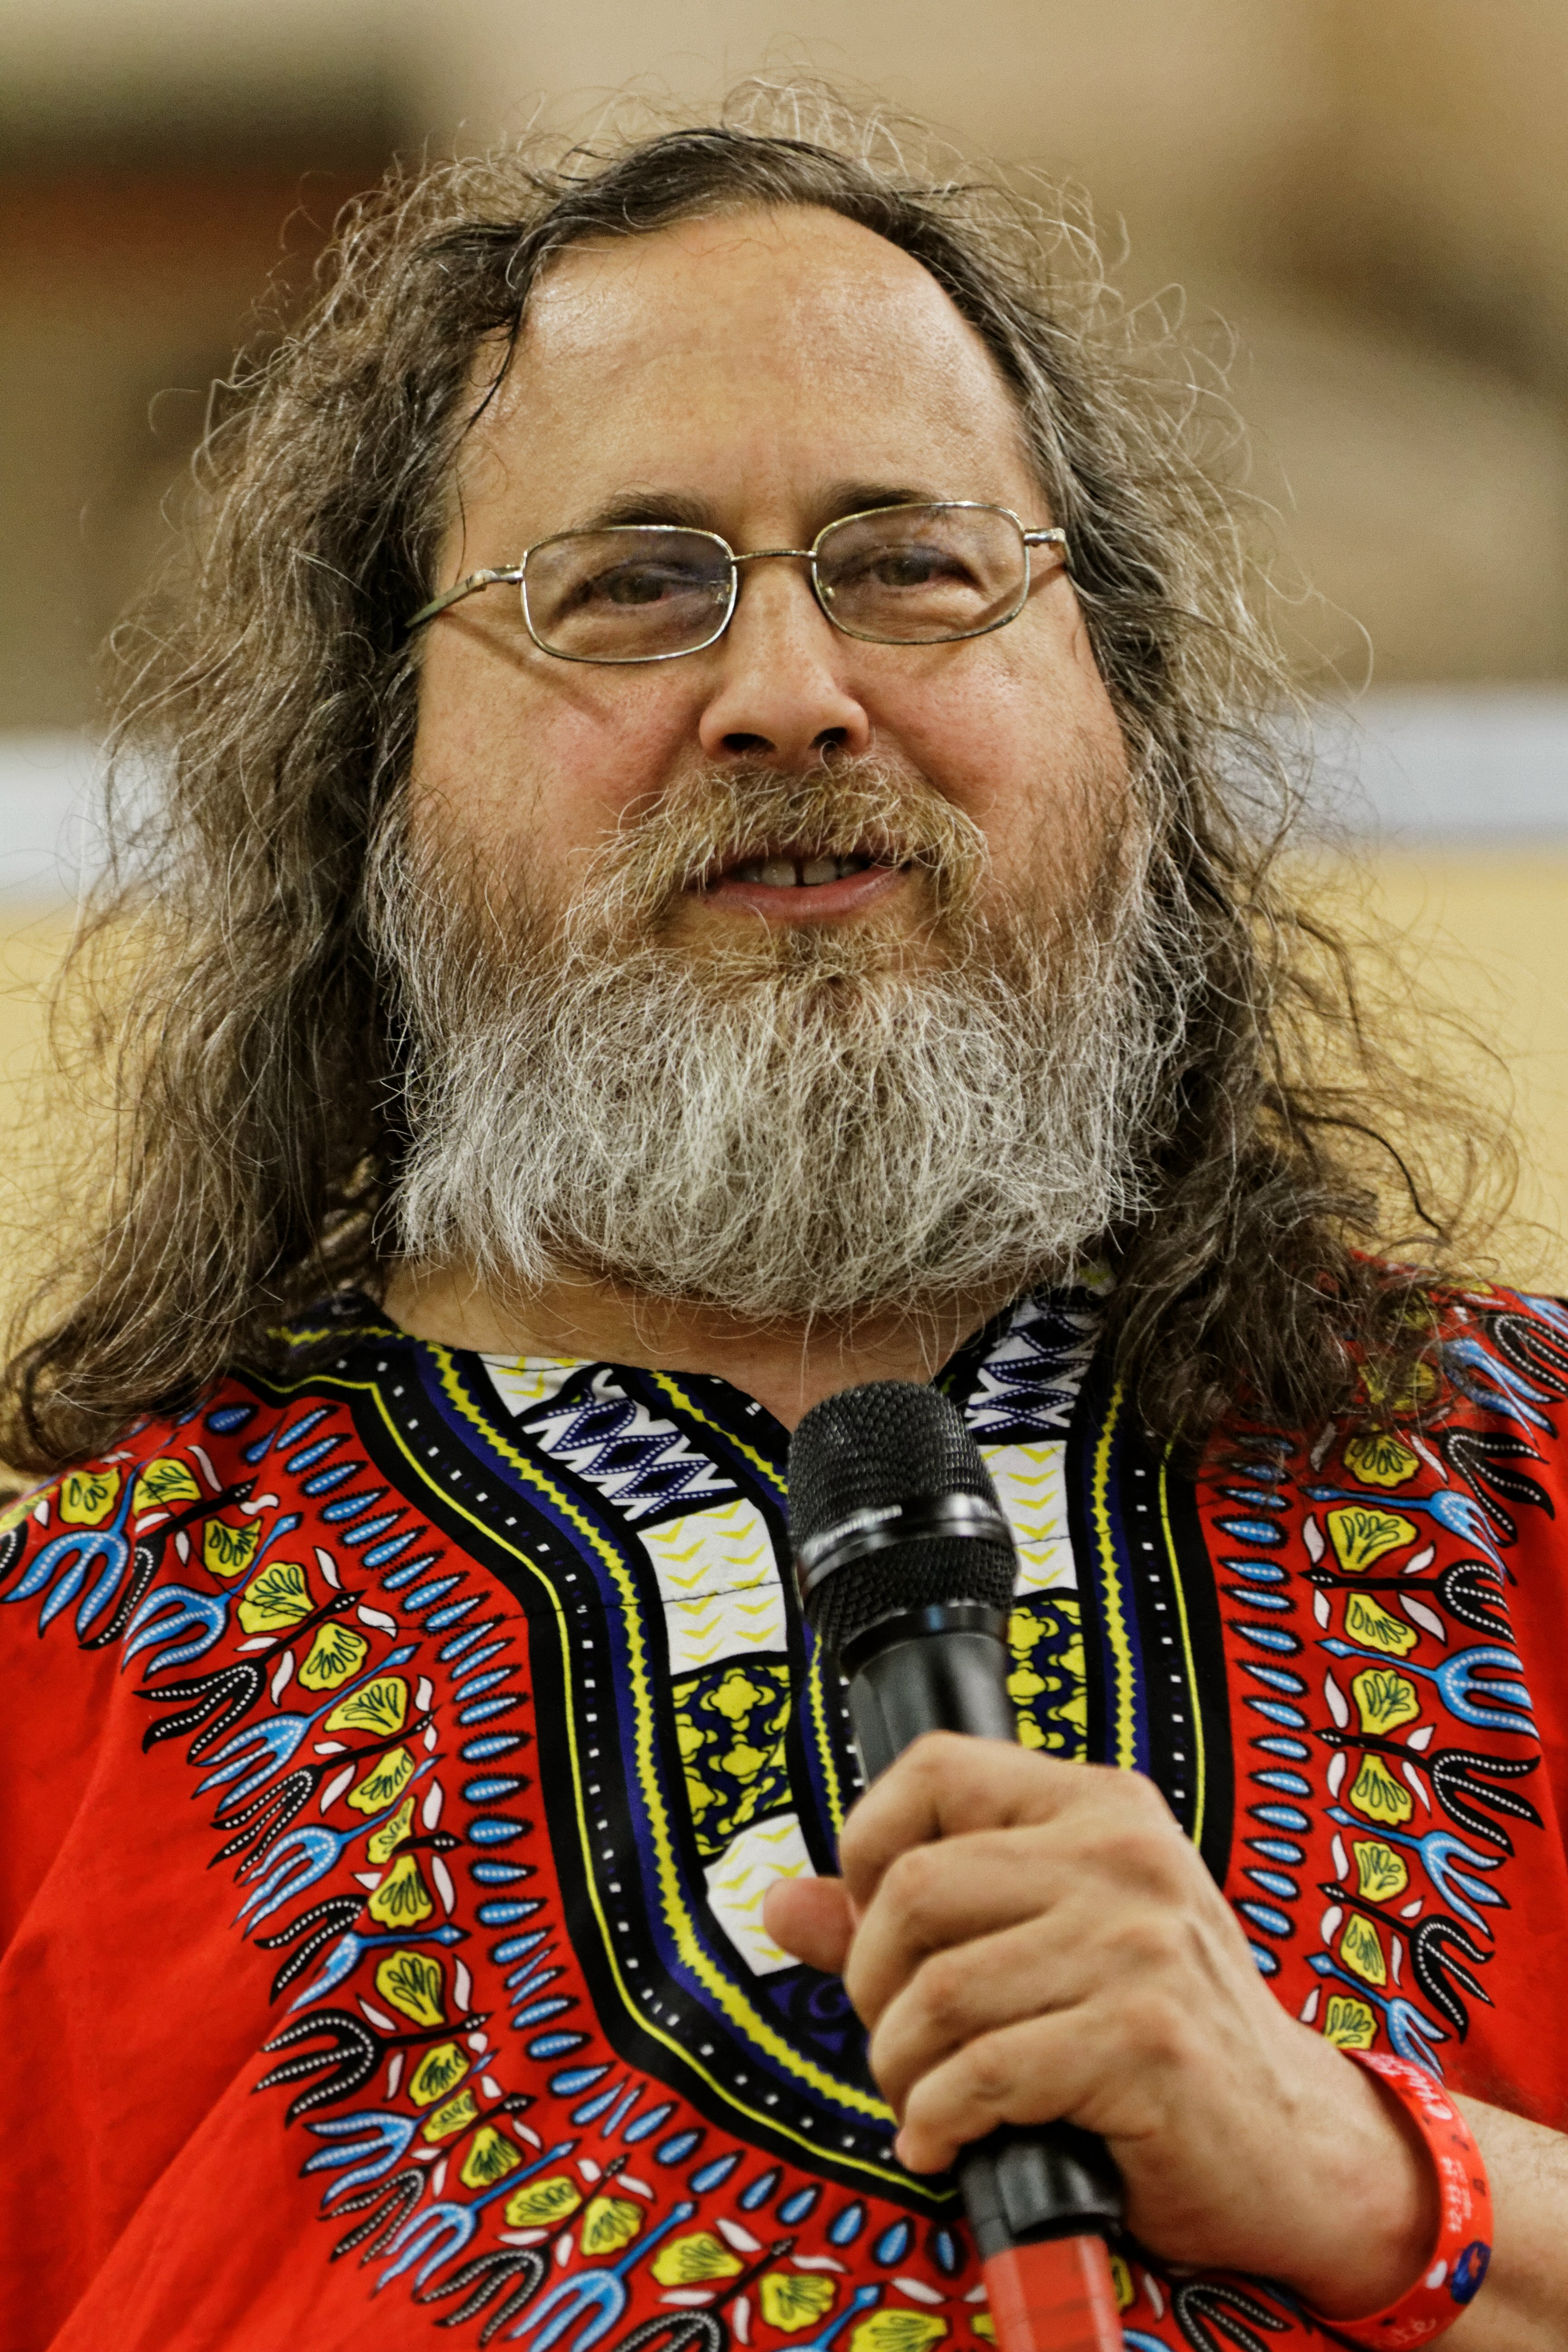
\includegraphics[width=.4\linewidth]{pic/stallman}};
    }
    \only<5-8>{
      \node at (-3,0)
        {
\includegraphics[width=.5\linewidth]{pic/poster}};

      \node at (3,0)
        {
\includegraphics[width=.5\linewidth]{pic/second}};
    }
    \only<6-8>{
      \node at (3,0)
        {
\includegraphics[width=.5\linewidth, trim={0 200 0 200}, clip]{pic/politics-second}};
    }
    \only<7-8>{
      \node at (-3,0)
        {
\includegraphics[width=.5\linewidth, trim={0 200 0 200}, clip]{pic/politics-poster}};
    }
    \only<8>{
      \node (t) [font=\bfseries\Huge, fill=white]
        {Reactionary politics is bad};

      \node[font=\bfseries\large, fill=white, above, align=center] at (t.north)
        {How should I say it guys};

      \node[font=\bfseries\large, fill=white, below, align=center, text width = .85\linewidth] at (t.south)
        {Political discourse ($\neq$ political progress) desperately needs to slow down. Read. Listen.};
    }
    \only<9->{
      \fill[white] (-7,4) rectangle (5,-5);
      \node (book) at (-5, 1) {
\includegraphics[width=.5\linewidth]{pic/dictator-handbook}};
      \node[below right, font=\bfseries\large, fill=white, text width=4cm] at (book.north east)
        {A recommendation if you are interested in politics};
      \node[above right, font=\large, fill=white, text width=5cm, anchor = south west] at (book.south east)
        {
          Simplified explaination of selectorate theory. Mostly about the
          \emph{structures} of power in politics than politics itself.
        };

      \node[below, anchor = north west, text width = \linewidth, fill=white] at (book.south west){
        Also: \emph{Eristic Dialectic} (Schopenhauer) \emph{Amusing Ourselves to
        Death} (Postman), \emph{Animal Farm} (Orwell), \emph{The Prince}
        (Machiavelli), and the many classics (Plato, Aristotle, Locke, Rousseau,
        Marx, Arendt, Rawls, Foucault, \ldots).
      };
    }
  \end{tikzpicture}
\end{frame}

% \begin{frame}{Social Acceleration I}
% 
%   \begin{quote}
%     She who lives twice as fast can realize twice as many worldly
%     possibilities, achieve two times as many goals, have twice as many
%     experiences, and accumulate twice as many lived events: she thus doubles
%     the amount of worldly options she exhausts. One who lives infinitely fast
%     no longer needs to fear death, the annihilator of options.
%   \end{quote}
% 
%   \begin{quote}
%     But the very same inventions, techniques, and methods that permit the
%     accelerated realization of worldly possibilities and hence the increase of
%     the total sum of options realized in a life, also multiply the number of
%     variety of relizable options in an exponential way. 
%   \end{quote}
% 
% \end{frame}
% 
% \begin{frame}{Social Acceleration II}
% 
%   \begin{quote}
%     Contrary to the promise of acceleration the degree of exhaustion, the ratio
%     of worldly possibilities realized in a life to those that are realizable,
%     continually decreases no matter how much we hurry around heightening the
%     tempo of our life. The modern strategy for realigning life time and worldly
%     time therefore backfires.
%   \end{quote}
%   
%   \begin{flushright}
%     --- Hartmut Rosa, Social Acceleration, 2005
%   \end{flushright}
%   
%   \vfill
% 
%   \begin{center}
%     \Large\bfseries
%     TL;DR: Slow the f*ck down.
%   \end{center}
%   \vfill
% \end{frame}

\section{The Solution}

\begin{frame}{Solving the Problem: Snapshots}
  \begin{center}
    \begin{tikzpicture}
    \node at (-1, 2) [draw, fill=gray!15, thick, font=\ttfamily, left] (P) {Project/};
    \pause
    \draw[black, thick, ->] (P.north east) ++(.2,-.2) arc (-90:180:.5)
        node[pos=.6, above]{Changes};
    \draw[black, thick, ->] (0, 0) -- (7.2, 0) node [below] {Time};
    \foreach \x/\t in {0/16:04:28, 2/16:37:01, 4/17:15:44, 6/18:01:03}
    {
        \pause
        \draw[color=black, fill=magenta, thick] (\x, 0) circle (.12)
            node[below=5pt, anchor=east, rotate=70, font=\ttfamily, align=right] {\tiny 2019-09-18\\\small\t};
        \draw[thick, ->, gray] (-.8, 2) to[bend left, in=120] (\x, .2);
    }
    \end{tikzpicture}
  \end{center}
\end{frame}

\subsection{Commit Graph}

\begin{frame}[fragile]{Solving the Problem: Concurrent Changes I}
  \begin{tikzpicture}[
      commit/.style = {
        draw, fill=orange, circle, thick,
        minimum size = 2.5mm, inner sep = 0, outer sep = 1mm,
      },
    ]
    \matrix (m) [
      column sep = 18mm, row sep = 1cm,
      row 2/.style = {row sep = 8mm},
    ] {
        \pic[visible on=<1->]{file = {fb0 f {}}}; 
      & \pic[visible on=<2->]{file = {fb1 f {}}}; 
      & \pic[visible on=<3->]{file = {fb2 f {}}}; 
      & \pic[visible on=<6->]{file = {fb3 f {}}}; 
      \\
        \node[visible on=<1->, commit, label={[visible on=<1->]60:A}] (cb0) {};
      & \node[visible on=<2->, commit, label={[visible on=<2->]60:B}] (cb1) {};
      & \node[visible on=<3->, commit, label={[visible on=<3->]60:C}] (cb2) {};
      & \node[visible on=<6->, commit, label={[visible on=<6->]60:M}, fill=magenta] (cb3) {};
        \only<6->{
          \fill[opacity=.2, magenta] (cb3) circle (5mm);
        }
      \\
      & \node[visible on=<4->, commit, label={[visible on=<4->]60:B'}] (ca1) {};
      & \node[visible on=<5->, commit, label={[visible on=<5->]60:C'}] (ca2) {};
      \\
        \pic[visible on=<3->]{file = {fa0 f {}}}; 
      & \pic[visible on=<4->]{file = {fa1 f {}}}; 
      & \pic[visible on=<5->]{file = {fa2 f {}}}; 
      & \pic[visible on=<6->]{file = {fa3 f {}}}; 
      \\
    };

    \node[rotate=90, font={\bfseries}, hsr-blue]  at ($(-.5,0) + (fb0.west)$) {Bob};
    \node[visible on=<3->, rotate=90, font={\bfseries}, hsr-mauve] at ($(-.5,0) + (fa0.west)$) {Alice};

    \begin{scope}[thick]
      \only<2->{
        \draw[->] (fb0) -- node[midway, above] {edit} (fb1);
        \draw[<-] (cb0) -- node[midway, above] {from} (cb1);
      }
      \only<3->{
        \draw[->] (fb1) -- node[midway, above] {edit} (fb2);
        \draw[<-] (cb1) -- node[midway, above] {from} (cb2);
      }

      \only<4->{
        \draw[->] (fa0) -- node[midway, above] {edit} (fa1);
        \draw[<-] (cb0) to[out=-60, in=180] 
                        node[midway, above, sloped] {from} (ca1);
      }

      \only<5->{
        \draw[->] (fa1) -- node[midway, above] {edit} (fa2);
        \draw[<-] (ca1) -- node[midway, above] {from} (ca2);
      }

      \only<6->{
        \draw[->] (fb2) -- node[midway, above] {``sync''} (fb3);
        \draw[<-] (cb2) -- node[midway, above] {from} (cb3);

        \draw[->] (fa2) -- node[midway, above] {``sync''} (fa3);
        \draw[<-] (ca2) to[out=0, in=-120]
                        node[midway, above, sloped] {from} (cb3);
      }

      \begin{scope}[gray]
        \draw[visible on=<1->, ->] (fb0) -- node[midway, left] {save} (cb0);
        \draw[visible on=<2->, ->] (fb1) -- node[midway, left] {save} (cb1);
        \draw[visible on=<3->, ->] (fb2) -- node[midway, left] {save} (cb2);

        \draw[visible on=<3->, ->] (cb0) -- node[midway, left] {copy} (fa0);
        \draw[visible on=<4->, ->] (fa1) -- node[midway, left] {save} (ca1);
        \draw[visible on=<5->, ->] (fa2) -- node[midway, left] {save} (ca2);

        \draw[visible on=<6->, ->] (cb3) -- node[midway, left] {copy} (fb3);
        \draw[visible on=<6->, ->] (cb3) -- node[midway, left] {copy} (fa3);
      \end{scope}
    \end{scope}
  \end{tikzpicture}
\end{frame}

\begin{frame}{Solving the Problem: Concurrent Changes II}
  \begin{block}{High Level Overview}
    Store changes using a \emph{directed acyclic graph} (DAG) called
    the \emph{commit graph}.
    \begin{itemize}
      \item Nodes are saved points in time called \emph{commits}
      \item Arcs point to state from which change was made
      \item Commits with multiple children (A) are \emph{branching commits}
      \item Commits with multiple parents (M) are \emph{merge commits}
    \end{itemize}
  \end{block}
  \begin{alertblock}{Problems}
    \begin{enumerate}
      \item We care about file content not the files itself
      \item How do we merge changes?
      \item Alice and Bob are not working on the same computer
    \end{enumerate}
  \end{alertblock}
\end{frame}

\subsection{Blobs and Trees}

\begin{frame}[fragile]{Solving the Problem: Multiple Files}
  \begin{columns}
    \begin{column}{.35\linewidth}
      \begin{tikzpicture}[
          grow via three points = {%
            one child at (0.8,-0.7) and %
              two children at (0.8,-0.7) and (0.8,-1.4)
          },
          edge from parent/.style = {draw,thick},
          edge from parent path = {
            ($(\tikzparentnode\tikzparentanchor)+(.4cm,0pt)$)
              |- (\tikzchildnode\tikzchildanchor)
          },
          growth parent anchor = west,
          parent anchor = south west,
          every node/.style = {
            anchor = west,
            font = \ttfamily,
          }
        ]
        \node {Project/}
          child { node {src/}
            child { node [draw=none, fill=none] {main.c} }
            child { node [draw=none, fill=none] {Makefile} }
            child { node {\ldots} }
          }
          child [missing] {}
          child [missing] {}
          child [missing] {}
          child { node {release/}
            child { node [draw=none, fill=none] {magic} }
            child { node [draw=none, fill=none] {awesome.a} }
          };
      \end{tikzpicture}
    \end{column}
    \begin{column}{.65\linewidth}
      \begin{block}{Filesystem Jargon}
        \begin{description}[wide]
          \item[Tree] Folder / Directory
          \item[Blob] Binary Large OBject, raw data (bits) of file
            content\footnote{Demo: \texttt{hexdump} vs \texttt{stat}}
          \item[File] Blob + Metadata (Name, Date, \ldots)
        \end{description}
      \end{block}
      \begin{alertblock}{Solution}
        Treat all blobs as single entity with metadata. Examples:
        \begin{itemize}
          \item Rename file $\Rightarrow$ Same blob, commit name change
          \item Move file $\Rightarrow$ Same blob, commit change tree
        \end{itemize}
      \end{alertblock}
    \end{column}
  \end{columns}
\end{frame}

\subsection{Branches}

\begin{frame}[fragile]{Mathematical Digression I: DAG}
  \begin{columns}
    \begin{column}{.55\linewidth}
      \begin{block}{Directed Acyclic Graph}
        A DAG $G = (V,A)$ is defined by a finite set of vertices $V$ and a
        finite set of \emph{arcs} $A$ and may not contain loops.
      \end{block}

      \begin{block}<2->{Partial Order}
        DAG have a partial order relation $u \succ v$ for comparable $u,v \in V$.
      \end{block}

      \begin{alertblock}<3->{Topological Order}
        A DAG $G = (V,A)$ has a total order $\succ^*$ by having that for all
        $(u, v) \in A$ $u \succ^* v$. If $G$ has a Hamiltonian path
        $\succ^*$
        is unique.
      \end{alertblock}
    \end{column}
    \begin{column}{.45\linewidth}
      \begin{tikzpicture}
        \matrix (m) [
          row sep = 5mm, column sep = 4mm,
          matrix of nodes, nodes = {
            circle, draw, thick, fill=orange,
            inner sep = 0pt, outer sep = 1mm, minimum size = 2.5mm,
          }
        ] {
          |[label={60:A}]| {} &                     \\
          |[label={60:B}]| {} &                      & |[label={60:C}]| {} \\
                              & |[label={90:D}]| {}  & |[label={60:E}]| {} \\
          |[label={90:F}]| {} &                      & |[label={60:G}]| {} \\
          |[label={60:H}]| {} & |[label={120:I}]| {}  &                     \\
                              & |[label={60:J}]| {} \\
        };

        \begin{scope}[thick, ->]
          \draw (m-1-1) -- (m-2-1);
          \draw (m-2-1) -- (m-3-2);
          \draw (m-3-2) -- (m-4-1);
          \draw (m-4-1) -- (m-5-1);
          \draw (m-5-1) -- (m-6-2);

          \draw (m-2-3) -- (m-3-2);

          \draw (m-1-1) -- (m-2-3);
          \draw (m-2-3) -- (m-3-3);
          \draw (m-3-3) -- (m-4-3);
          \draw (m-4-3) -- (m-5-2);
          \draw (m-5-2) -- (m-6-2);

          \draw (m-3-2) -- (m-5-2);
        \end{scope}
        
        \only<3->{
          \matrix (s) [
            right = 7mm of m,
            row sep = 4mm,
            matrix of nodes, nodes = {
              circle, draw, thick, fill=orange,
              inner sep = 0pt, outer sep = 1mm, minimum size = 2.5mm,
            }
          ] {
            |(A) [label={0:A}]| {} \\ 
            |(C) [label={0:C}]| {} \\ 
            |(B) [label={0:B}]| {} \\ 
            |(E) [label={0:E}]| {} \\ 
            |(D) [label={0:D}]| {} \\ 
            |(G) [label={0:G}]| {} \\ 
            |(F) [label={0:F}]| {} \\ 
            |(I) [label={0:I}]| {} \\ 
            |(H) [label={0:H}]| {} \\ 
            |(J) [label={0:J}]| {} \\
          };
          
          \begin{scope}[thick, ->]
            \draw (A) to[bend left] (B);
            \draw (A) to (C);
            \draw (B) to[bend left] (D);
            \draw (C) to[bend right] (D);
            \draw (C) to[bend right] (E);
            \draw (D) to[bend left] (F);
            \draw (D) to[bend right] (I);
            \draw (E) to[bend right] (G);
            \draw (F) to[bend left] (H);
            \draw (G) to[bend right] (I);
            \draw (H) to (J);
            \draw (I) to[bend right] (J);
          \end{scope}
        }
      \end{tikzpicture}
    \end{column}
  \end{columns}
\end{frame}

\begin{frame}[fragile]{Solving the Problem: Concurrent Changes III}
  \begin{columns}[t]
    \begin{column}{\linewidth}
      \centering
      \begin{tikzpicture}
        \matrix (m) [
          column sep = 8mm, row sep = 8mm,
          matrix of nodes, nodes = {
            circle, draw, thick, fill=orange,
            inner sep = 0pt, outer sep = 1mm, minimum size = 2.5mm,
          },
        ] {
          & |[fill=magenta]| {}
          & |[fill=magenta]| {}
          & |[fill=magenta]| {}
          &
          &
          & |[fill=hsr-blue]| {}
          & |[fill=hsr-blue]| {}
          &
          \\
          |[fill=lightgray]| {} 
          &    
          & {} 
          &    
          & {} 
          & {} 
          & {} 
          &
          & {}
          & {}
          \\
          &    
          &    
          & |[fill=teal]| {} 
          & |[fill=teal]| {} 
          & |[fill=teal]| {} 
          &    
          & |[fill=teal]| {} 
          & |[fill=teal]| {}
          \\
        };

        \begin{scope}[thick, <-]
          \draw (m-2-1) -- (m-1-2);

          % above first
          \draw (m-1-2) -- (m-1-3);
          \draw (m-1-3) -- (m-1-4);
          \draw (m-1-4) -- (m-2-5);

          % middle
          \draw (m-2-1) -- (m-2-3);
          \draw (m-2-3) -- (m-2-5);
          \draw (m-2-5) -- (m-2-6);
          \draw (m-2-6) -- (m-2-7);
          \draw (m-2-7) -- (m-2-9);
          \draw (m-2-9) -- (m-2-10);

          % below
          \draw (m-2-3) -- (m-3-4);
          \draw (m-3-4) -- (m-3-5);
          \draw (m-3-5) -- (m-3-6);
          \draw (m-3-6) -- (m-3-8);
          \draw (m-2-7) -- (m-3-8); % merge
          \draw (m-3-8) -- (m-3-9);

          % above second
          \draw (m-2-6) -- (m-1-7);
          \draw (m-1-7) -- (m-1-8);
        \end{scope}

        \node[right = 2mm, font=\ttfamily, visible on=<2->] at (m-1-8) {quickfix};
        \node[above = 2mm, font=\ttfamily, visible on=<2->] at (m-2-10) {master};
        \node[above = 2mm, font=\ttfamily, visible on=<2->] at (m-3-9) {feature};
      \end{tikzpicture}
    \end{column}
  \end{columns}

  \begin{columns}[t]
    \begin{column}{.5\linewidth}
      \begin{block}{Branch (informal)}
        Branches are subgraphs (subtrees) from a common anchestor in the commit
        graph.
      \end{block}
      \begin{alertblock}{Naming Branches}<2->
        Branch names are labels on their most recent commit.
      \end{alertblock}
    \end{column}
    \begin{column}{.5\linewidth}
      \begin{exampleblock}{Examples}<3->
        \begin{itemize}
          \item \texttt{quickfix} branch is from \texttt{master}
          \item Magenta (no name) branch was merged into \texttt{master}
          \item \texttt{master} branch was merged into \texttt{feature}
        \end{itemize}
      \end{exampleblock}
    \end{column}
  \end{columns}
\end{frame}

\subsection{Merging Strategies}

\begin{frame}[fragile]{Solving the Problem: Fast-Forward-Merge}
  \begin{columns}
    \begin{column}{.5\linewidth}
      \begin{tikzpicture}
        \matrix (m) [
          column sep = 8mm, row sep = 6mm,
          fill = lightgray!20, inner sep = 5mm, outer sep = 2mm,
          matrix of nodes, nodes = {
            circle, draw, thick, fill=orange,
            inner sep = 0pt, outer sep = 1mm, minimum size = 2.5mm,
          },
          row 1/.style = {
            nodes = {
              fill = magenta,
            }
          }
        ] {
             &    & {} & {} & {} \\
          {} & {} & \\
        };

        \begin{scope}[thick, <-]
          \draw (m-2-1) -- (m-2-2);
          \draw (m-2-2) -- (m-1-3);
          \draw (m-1-3) -- (m-1-4);
          \draw (m-1-4) -- (m-1-5);
        \end{scope}

        \begin{scope}[font=\ttfamily]
          \node[below = 1mm] at (m-2-2) {BX};
          \node[above = 1mm] at (m-1-5) {BY};
        \end{scope}

        \matrix (n) [visible on=<2->,
          below = 2cm of m,
          column sep = 8mm, row sep = 6mm,
          fill = lightgray!20, inner sep = 5mm, outer sep = 2mm,
          matrix of nodes, nodes = {
            circle, draw, thick, fill=magenta,
            inner sep = 0pt, outer sep = 1mm, minimum size = 2.5mm,
          },
        ] {
          |[fill=orange]| {} & |[fill=orange]| {} & {} & {} & {} \\
        };

        \only<2->{
          \begin{scope}[thick, <-]
            \draw (n-1-1) -- (n-1-2);
            \draw (n-1-2) -- (n-1-3);
            \draw (n-1-3) -- (n-1-4);
            \draw (n-1-4) -- (n-1-5);
          \end{scope}

          \begin{scope}[font=\ttfamily]
            \node[below = 1mm] at (n-1-5) {BX};
            \node[above = 1mm] at (n-1-5) {BY};
          \end{scope}

          \draw[very thick, ->] (m) -- node[midway, right]
            {in \texttt{BX} merge \texttt{BY}} (n);
        }
      \end{tikzpicture}
    \end{column}
    \begin{column}{.5\linewidth}
      \begin{exampleblock}{History}
        \begin{enumerate}
          \item From an existing branch \texttt{BX} (with orange commits) a
            branch \texttt{BY} added new commits (magenta)
          \item We merge \texttt{BY} into \texttt{BX}
        \end{enumerate}
      \end{exampleblock}
      \begin{alertblock}<2->{FF-Merge}
        Apply changes of commits in \texttt{BY} starting at \texttt{BX} until
        you get to \texttt{BY}. Or \texttt{BX} just needs to ``catch up'' to
        \texttt{BY}. No new commits are created.
      \end{alertblock}
    \end{column}
  \end{columns}
\end{frame}

\begin{frame}[fragile]{Solving the Problem: 3-Way-Merge I}
  \begin{columns}
    \begin{column}{.5\linewidth}
      \begin{tikzpicture}
        \matrix (m) [
          column sep = 8mm, row sep = 6mm,
          fill = lightgray!20, inner sep = 5mm, outer sep = 2mm,
          matrix of nodes, nodes = {
            circle, draw, thick, fill=orange,
            inner sep = 0pt, outer sep = 1mm, minimum size = 2.5mm,
          },
          row 1/.style = {
            nodes = {
              fill = magenta,
            }
          }
        ] {
             &    & {} & {} \\
          {} & {} & |[fill=teal]| {} \\
        };

        \begin{scope}[thick, <-]
          \draw (m-2-1) -- (m-2-2);
          \draw (m-2-2) -- (m-1-3);
          \draw (m-1-3) -- (m-1-4);

          \draw (m-2-2) -- (m-2-3);
        \end{scope}

        \begin{scope}[font=\ttfamily]
          \node[below = 1mm] at (m-2-3) {BX};
          \node[above = 1mm] at (m-1-4) {BY};
        \end{scope}

        \matrix (n) [visible on=<2->,
          below = 2cm of m,
          column sep = 8mm, row sep = 6mm,
          fill = lightgray!20, inner sep = 5mm, outer sep = 2mm,
          matrix of nodes, nodes = {
            circle, draw, thick, fill=orange,
            inner sep = 0pt, outer sep = 1mm, minimum size = 2.5mm,
          },
        ] {
             &    & |[fill=magenta]| {} & |[fill=magenta]| {} \\
          {} & {} & |[fill=teal]| {} & & |[fill=hsr-blue]| {} \\
        };

        \only<2->{
          \begin{scope}[thick, <-]
            \draw (n-2-1) -- (n-2-2);
            \draw (n-2-2) -- (n-1-3);
            \draw (n-1-3) -- (n-1-4);
            \draw (n-1-4) -- (n-2-5);

            \draw (n-2-2) -- (n-2-3);
            \draw (n-2-3) -- (n-2-5);
          \end{scope}

          \begin{scope}[font=\ttfamily]
            \node[below = 1mm] at (n-2-5) {BX};
            \node[above = 1mm] at (n-1-4) {BY};
          \end{scope}

          \draw[very thick, ->] (m) -- node[midway, right]
            {in \texttt{BX} merge \texttt{BY}} (n);
        }
      \end{tikzpicture}
    \end{column}
    \begin{column}{.5\linewidth}
      \begin{exampleblock}{History}
        \begin{enumerate}
          \item Branches \texttt{BX} and \texttt{BY} have new commits (magenta
            and green resp.) and share a common history (orange)
          \item We merge \texttt{BY} into \texttt{BX}
        \end{enumerate}
      \end{exampleblock}
      \begin{alertblock}<2->{Observations}
        When you merge you are in \texttt{BX} importing changes from \texttt{BY}
        \begin{itemize}
          \item ``our'' changes are from \texttt{BX}
          \item ``their'' changes are from \texttt{BY}
        \end{itemize}
        Need to make choices, which get saved in a new merge commit.
      \end{alertblock}
    \end{column}
  \end{columns}
\end{frame}

\begin{frame}[fragile]{Solving the Problem: 3-Way-Merge II}
  \begin{columns}
    \begin{column}{.55\linewidth}
      \begin{tikzpicture}
        \node[draw, very thick, teal, fill=teal!20,
          circle, minimum size = 20mm] (oc) {};

        \node[draw, very thick, magenta, fill=magenta!20, 
          circle, minimum size = 20mm, right = 15mm of oc] (tc) {};

        \node[above right = 1cm, font=\ttfamily] at (oc) {BX};
        \node[above right = 1cm, font=\ttfamily] at (tc) {BY};

        \draw (oc) pic{file = {of ours {}}};
        \draw (tc) pic{file = {tf theirs {}}};

        \begin{scope}
          \clip (oc) circle[radius=1cm];
          \node[opacity=.08] at (oc) {
            
\includegraphics[width=3cm]{pic/ours}
          };
        \end{scope}

        \node[draw, very thick, hsr-blue, fill=hsr-blue20,
          rounded corners = 5mm, minimum width = 5cm, minimum height = 2cm]
          (mc) at ($(oc)!0.5!(tc) - (0,4)$) {};

        \node[draw, thick, black, fill = white,
          minimum width = 4cm, minimum height = 1cm,]
          (mf) at (mc) {merged};

        \node[below] at (mc.south) {Merge \texttt{BY} into \texttt{BX}};

        \begin{scope}[black, line width = 1mm]
          \draw[<-] (oc.south) -- (mc);
          \draw[<-] (tc.south) -- (mc);
          \draw[] (oc.north) -- ++ (0,1);
          \draw[] (tc.north) -- ++ (0,1);
        \end{scope}

        \foreach \k/\w [count=\i] in {0/9, 1.2/5, 2.3/6, 3.2/2} {
          \node[draw, thick, teal, fill=teal!40,
            minimum height = 1cm, minimum width = \w,
            opacity = .5, inner sep = 0pt, anchor = west,
          ] (moc-\i) at ($(mf.west) + (\k,0)$) {};
          
          \draw[teal, thick, ->] (of) to[out=-90, in=90] ({moc-\i}.north);
        }

        \foreach \k/\w [count=\i] in {.6/2, 1.4/9, 3/4} {
          \node[draw, thick, magenta, fill=magenta!40,
            minimum height = 1cm, minimum width = \w,
            opacity = .5, inner sep = 0pt, anchor = west,
          ] (mtc-\i) at ($(mf.west) + (\k,0)$) {};

          \draw[magenta, thick, ->] (tf) to[out=-90, in=90] ({mtc-\i}.north);
        }
      \end{tikzpicture}
    \end{column}
    \begin{column}{.45\linewidth}
      \begin{alertblock}{3-Way-Merge}
        \begin{itemize}
          \item Use a (3-way-merge) algorithm to merge trees and blobs from
            each commit

          \item If not possible the user has to choose between `our' changes
            and `their' changes
        \end{itemize}
      \end{alertblock}
      \begin{block}{Merge Conflict}
        When the algorithm cannot merge the file automatically it is called
        \emph{merge conflict}.
      \end{block}
    \end{column}
  \end{columns}
\end{frame}

\begin{frame}[fragile]{Solving the Problem: Rebase}
  \begin{columns}
    \begin{column}{.5\linewidth}
      \begin{tikzpicture}
        \matrix (m) [
          column sep = 8mm, row sep = 6mm,
          fill = lightgray!20, inner sep = 5mm, outer sep = 2mm,
          matrix of nodes, nodes = {
            circle, draw, thick, fill=orange,
            inner sep = 0pt, outer sep = 1mm, minimum size = 2.5mm,
          },
          row 1/.style = {
            nodes = {
              fill = magenta,
            }
          }
        ] {
             &    & {} & {} \\
          {} & {} & |[fill=teal]| {} \\
        };

        \begin{scope}[thick, <-]
          \draw (m-2-1) -- (m-2-2);
          \draw (m-2-2) -- (m-1-3);
          \draw (m-1-3) -- (m-1-4);

          \draw (m-2-2) -- (m-2-3);
        \end{scope}

        \begin{scope}[font=\ttfamily]
          \node[below = 1mm] at (m-2-3) {BX};
          \node[above = 1mm] at (m-1-4) {BY};
        \end{scope}

        \matrix (n) [visible on=<2->,
          below = 2cm of m,
          column sep = 8mm, row sep = 6mm,
          fill = lightgray!20, inner sep = 5mm, outer sep = 2mm,
          matrix of nodes, nodes = {
            circle, draw, thick, fill=orange,
            inner sep = 0pt, outer sep = 1mm, minimum size = 2.5mm,
          },
        ] {
          {} & {} & |[fill=teal]| {} & |[fill=magenta]| {} & |[fill=magenta]| {}  \\
        };

        \only<2->{
          \begin{scope}[thick, <-]
            \draw (n-1-1) -- (n-1-2);
            \draw (n-1-2) -- (n-1-3);
            \draw (n-1-3) -- (n-1-4);
            \draw (n-1-4) -- (n-1-5);
          \end{scope}

          \begin{scope}[font=\ttfamily]
            \node[below = 1mm] at (n-1-5) {BX};
            \node[above = 1mm] at (n-1-5) {BY};
          \end{scope}

          \draw[very thick, ->] (m) -- node[midway, right]
            {in \texttt{BX} rebase \texttt{BY}} (n);
        }
      \end{tikzpicture}
    \end{column}
    \begin{column}{.5\linewidth}
      \begin{exampleblock}{History}
        \begin{enumerate}
          \item Branches \texttt{BX} and \texttt{BY} have new commits (magenta
            and green resp.) and share a common history (orange)
          \item We rebase \texttt{BY} onto \texttt{BX}
        \end{enumerate}
      \end{exampleblock}
      \begin{alertblock}<2->{Observations}
        When you rebase you need to reapply your changes on the newer versions
        of the files. Hence you may need to resolve some conflicts during this process.
      \end{alertblock}
    \end{column}
  \end{columns}
\end{frame}

\subsection{Remotes}

\begin{frame}[fragile]{Solving the Problem: Multiple Computers I}
  \begin{columns}
    \begin{column}{.6\linewidth}
      \centering
      \begin{tikzpicture}

        \matrix (b) [
          row sep = 6mm, column sep = 6mm, 
          outer sep = 3mm, inner sep = 6mm,
          matrix of nodes, nodes = {
            draw, thick, circle, fill = teal,
            inner sep = 0pt, outer sep = .5mm, minimum size = 2mm,
          },
          draw = hsr-blue, thick, fill=hsr-blue20,
        ] {
          {} & {} &    & {} & |[fill=hsr-blue, visible on=<3->]| {} & |[fill=hsr-blue, visible on=<3->]| {} \\
             & {} & {} \\
        };
        \node[
          above, anchor = south, rotate = 90,
          font = \bfseries, text = hsr-blue,
        ] at (b.west) {Bob's PC};

        \begin{scope}[thick, <-]
          \draw (b-1-1) -- (b-1-2);
          \draw (b-1-2) -- (b-1-4);

          \draw (b-1-1) -- (b-2-2);
          \draw (b-2-2) -- (b-2-3);

          \only<3->{
            \draw[densely dashed] (b-1-4) -- (b-1-5);
            \draw[densely dashed] (b-1-5) -- (b-1-6);
          }
        \end{scope}

        \only<1-2>{
          \node[right = 2mm, font = \ttfamily] at (b-1-4) {trunk};
        }
        \only<3->{
          \node[above = 2mm, font = \ttfamily] at (b-1-6) {trunk};
        }
        \node[right = 2mm, font = \ttfamily] at (b-2-3) {feat};

        \matrix (a) [visible on=<2->,
          below = 16mm of b,
          row sep = 6mm, column sep = 6mm,
          outer sep = 3mm, inner sep = 6mm,
          matrix of nodes, nodes = {
            draw, thick, circle, fill = teal,
            inner sep = 0pt, outer sep = .5mm, minimum size = 2mm,
          },
          draw = hsr-mauve, thick, fill=hsr-mauve20,
        ] {
          {} & {} &    & {} \\
             & {} & {} &    & |[fill=hsr-mauve, visible on=<3->]| {} & |[fill=hsr-mauve, visible on=<3->]| {} \\
        };
        \only<2->{
          \node[
            above, anchor = south, rotate = 90,
            font = \bfseries, text = hsr-mauve,
          ] at (a.west) {Alice's PC};

          \begin{scope}[thick, <-]
            \draw (a-1-1) -- (a-1-2);
            \draw (a-1-2) -- (a-1-4);

            \draw (a-1-1) -- (a-2-2);
            \draw (a-2-2) -- (a-2-3);

            \only<3->{
              \draw[densely dashed] (a-1-4) -- (a-2-5);
              \draw[densely dashed] (a-2-3) -- (a-2-5);
              \draw[densely dashed] (a-2-5) -- (a-2-6);
            }
          \end{scope}

          \only<2>{
            \node[right = 2mm, font = \ttfamily] at (a-1-4) {trunk};
            \node[right = 2mm, font = \ttfamily] at (a-2-3) {feat};
          }
          \only<3->{
            \node[above = 2mm, font = \ttfamily] at (a-1-4) {trunk};
            \node[above = 2mm, font = \ttfamily] at (a-2-6) {feat};
          }

          \draw [very thick, hsr-mauve, ->] (b) -- node[midway, right] {clone} (a);
        }
      \end{tikzpicture}
    \end{column}
    \begin{column}{.4\linewidth}
      \begin{block}{Remotes and Clone}
        \footnotesize
        Other computers are called \emph{remotes}. Clone means you copy the
        commit graph on the remote machine onto yours.
      \end{block}
      \begin{exampleblock}{Example}
        \footnotesize
        \begin{enumerate}
          \item Alice has cloned Bob's (green) commit graph 
          \item Alice has merged \texttt{trunk} onto \texttt{feat} and made changes
          \item Bob has also made changes on \texttt{trunk}
        \end{enumerate}
      \end{exampleblock}
    \end{column}
  \end{columns}
\end{frame}

\begin{frame}[fragile]{Solving the Problem: Multiple Computers II}
  \begin{columns}
    \begin{column}{.6\linewidth}
      \centering
      \begin{tikzpicture}

        \matrix (b) [
          row sep = 6mm, column sep = 6mm, 
          outer sep = 1mm, inner sep = 6mm,
          minimum width = 6cm,
          matrix of nodes, nodes = {
            draw, thick, circle, fill = teal,
            inner sep = 0pt, outer sep = .5mm, minimum size = 2mm,
          },
          draw = hsr-blue, thick, fill=hsr-blue20,
        ] {
          {} & {} &    & {} & |[fill=hsr-blue]| {} & |[fill=hsr-blue]| {} \\
             & {} & {} \\
        };

        \node[
          above, anchor = south, rotate = 90,
          font = \bfseries, text = hsr-blue,
        ] at (b.west) {Bob's PC};

        \node[
          anchor = south west,
          font = \ttfamily, text = hsr-blue,
        ] at (b.north west) {bob};

        \begin{scope}[thick, <-]
          \draw (b-1-1) -- (b-1-2);
          \draw (b-1-2) -- (b-1-4);

          \draw (b-1-1) -- (b-2-2);
          \draw (b-2-2) -- (b-2-3);

          \draw (b-1-4) -- (b-1-5);
          \draw (b-1-5) -- (b-1-6);
        \end{scope}

        \node[above = 2mm, font = \footnotesize\ttfamily] (bt) at (b-1-6) {trunk};
        \node[right = 2mm, font = \footnotesize\ttfamily] (bf) at (b-2-3) {feat};

        \matrix (a) [
          below = 16mm of b,
          row sep = 6mm, column sep = 6mm,
          outer sep = 1mm, inner sep = 6mm,
          minimum width = 6cm,
          matrix of nodes, nodes = {
            draw, thick, circle, fill = teal,
            inner sep = 0pt, outer sep = .5mm, minimum size = 2mm,
          },
          draw = hsr-mauve, thick, fill=hsr-mauve20,
        ] {
          {} & {} &    & {} & |[fill=hsr-blue]| {}  & |[fill=hsr-blue]| {}  \\
             & {} & {} &    & |[fill=hsr-mauve]| {} & |[fill=hsr-mauve]| {} \\
        };

        \node[
          above, anchor = south, rotate = 90,
          font = \bfseries, text = hsr-mauve,
        ] at (a.west) {Alice's PC};

        \node[
          anchor = south west,
          font = \ttfamily, text = hsr-mauve,
        ] at (a.north west) {alice};

        \begin{scope}[thick, <-]
          \draw (a-1-1) -- (a-1-2);
          \draw (a-1-2) -- (a-1-4);

          \draw (a-1-1) -- (a-2-2);
          \draw (a-2-2) -- (a-2-3);

          \draw (a-1-4) -- (a-2-5);
          \draw (a-2-3) -- (a-2-5);
          \draw (a-2-5) -- (a-2-6);

          \draw (a-1-4) -- (a-1-5);
          \draw (a-1-5) -- (a-1-6);
        \end{scope}

        \node[above = 2mm, font = \footnotesize\ttfamily] at (a-1-4) {trunk};
        \node[below = 2mm, font = \footnotesize\ttfamily] at (a-2-6) {feat};

        \node[above = 2mm, font = \footnotesize\ttfamily, hsr-blue] (rbt) at (a-1-6) {bob/trunk};
        \node[below = 2mm, font = \footnotesize\ttfamily, hsr-blue] (rbf) at (a-2-3) {bob/feat};

        \begin{scope}[very thick, dashed, opacity=.5, gray, ->]
          \draw (bt.south east) to[bend left] (rbt.north east);
          \draw (bf) to[bend right] (rbf);
          \draw (b-1-6) to[bend right] (a-1-6);
          \draw (b-1-5) to[bend right] (a-1-5);
        \end{scope}

        \draw[very thick, ->, hsr-mauve] (b.south) -- 
          node[midway, right, fill=white] {fetch} (a.north);

      \end{tikzpicture}
    \end{column}
    \begin{column}{.4\linewidth}
      \begin{block}{Fetch}
        Copy the changes of the remote git graph into your local git graph.
      \end{block}
      \begin{exampleblock}{Running Example}
        Alice fetches Bob's changes.
      \end{exampleblock}
      \begin{alertblock}{Remote Branches}
        \footnotesize
        A branch that represents changes done in another machine. When a graph
        is cloned, the machine from which it was cloned has the default name
        \texttt{origin}.
      \end{alertblock}
    \end{column}
  \end{columns}
\end{frame}

\begin{frame}[fragile]{Solving the Problem: Multiple Computers III}
  \begin{columns}
    \begin{column}{.6\linewidth}
      \centering
      \begin{tikzpicture}

        \matrix (b) [
          row sep = 6mm, column sep = 6mm, 
          outer sep = 1mm, inner sep = 6mm,
          minimum width = 6cm,
          matrix of nodes, nodes = {
            draw, thick, circle, fill = teal,
            inner sep = 0pt, outer sep = .5mm, minimum size = 2mm,
          },
          draw = hsr-blue, thick, fill=hsr-blue20,
        ] {
          {} & {} &    & {} & |[fill=hsr-blue]| {}  & |[fill=hsr-blue]| {}  \\
             & {} & {} &    & |[fill=hsr-mauve]| {} & |[fill=hsr-mauve]| {} \\
        };

        \node[
          above, anchor = south, rotate = 90,
          font = \bfseries, text = hsr-blue,
        ] at (b.west) {Bob's PC};

        \node[
          anchor = south west,
          font = \ttfamily, text = hsr-blue,
        ] at (b.north west) {bob};

        \begin{scope}[thick, <-]
          \draw (b-1-1) -- (b-1-2);
          \draw (b-1-2) -- (b-1-4);

          \draw (b-1-1) -- (b-2-2);
          \draw (b-2-2) -- (b-2-3);

          \draw (b-1-4) -- (b-2-5);
          \draw (b-2-3) -- (b-2-5);
          \draw (b-2-5) -- (b-2-6);

          \draw (b-1-4) -- (b-1-5);
          \draw (b-1-5) -- (b-1-6);
        \end{scope}

        \node[above = 2mm, font = \footnotesize\ttfamily] at (b-1-6) {trunk};
        \node[below = 2mm, font = \footnotesize\ttfamily] at (b-2-3) {feat};

        \node[above = 2mm, font = \footnotesize\ttfamily, hsr-mauve] (rat) at (b-1-4) {alice/trunk};
        \node[below = 2mm, font = \footnotesize\ttfamily, hsr-mauve] (raf) at (b-2-6) {alice/feat};

        \matrix (a) [
          below = 16mm of b,
          row sep = 6mm, column sep = 6mm,
          outer sep = 1mm, inner sep = 6mm,
          minimum width = 6cm,
          matrix of nodes, nodes = {
            draw, thick, circle, fill = teal,
            inner sep = 0pt, outer sep = .5mm, minimum size = 2mm,
          },
          draw = hsr-mauve, thick, fill=hsr-mauve20,
        ] {
          {} & {} &    & {} & |[fill=hsr-blue]| {}  & |[fill=hsr-blue]| {}  \\
             & {} & {} &    & |[fill=hsr-mauve]| {} & |[fill=hsr-mauve]| {} \\
        };

        \node[
          above, anchor = south, rotate = 90,
          font = \bfseries, text = hsr-mauve,
        ] at (a.west) {Alice's PC};

        \node[
          anchor = south west,
          font = \ttfamily, text = hsr-mauve,
        ] at (a.north west) {alice};

        \begin{scope}[thick, <-]
          \draw (a-1-1) -- (a-1-2);
          \draw (a-1-2) -- (a-1-4);

          \draw (a-1-1) -- (a-2-2);
          \draw (a-2-2) -- (a-2-3);

          \draw (a-1-4) -- (a-2-5);
          \draw (a-2-3) -- (a-2-5);
          \draw (a-2-5) -- (a-2-6);

          \draw (a-1-4) -- (a-1-5);
          \draw (a-1-5) -- (a-1-6);
        \end{scope}

        \node[above = 2mm, font = \footnotesize\ttfamily] (at) at (a-1-4) {trunk};
        \node[below = 2mm, font = \footnotesize\ttfamily] (af) at (a-2-6) {feat};

        \node[above = 2mm, font = \footnotesize\ttfamily, hsr-blue] at (a-1-6) {bob/trunk};
        \node[below = 2mm, font = \footnotesize\ttfamily, hsr-blue] at (a-2-3) {bob/feat};

        \begin{scope}[very thick, dashed, opacity=.5, gray, ->]
          \draw (at.north west) to[bend left] (rat.south west);
          \draw (af.north east) to[bend right] (raf.south east);

          \draw (a-2-5) to[bend right] (b-2-5);
          \draw (a-2-6) to[bend right] (b-2-6);
        \end{scope}

        \draw[very thick, <-, hsr-mauve] ($(b.south) + (.1,0)$)
          -- node[midway, right, fill=white] {push} ($(a.north) + (.1,0)$);

        \draw[very thick, <-, hsr-blue] ($(b.south) - (.1,0)$)
          -- node[midway, left, fill=white] {fetch} ($(a.north) - (.1,0)$);

      \end{tikzpicture}
    \end{column}
    \begin{column}{.4\linewidth}
      \begin{block}{Push}
        Copy the changes of your local git graph to the remote machine.
      \end{block}

      \begin{exampleblock}{Running Example}
        This is the same as if Bob had fetched Alice's changes.
      \end{exampleblock}

      \begin{alertblock}{Network Access}
        \footnotesize
        In practice you cannot directly access other people's machines, so
        people use a third computer to which both parties have access (more
        later).
      \end{alertblock}
    \end{column}
  \end{columns}
\end{frame}

\begin{frame}[fragile]{Solving the Problem: Multiple Computers IV}
  \begin{columns}
    \begin{column}{1.1\linewidth}
      Since it is very a common operation there is a shorthand to fetch and
      merge the remote branch with the same name as the current one.

      \begin{center}
        \noindent
        \begin{tikzpicture}
          \matrix (b) [
            row sep = 6mm, column sep = 6mm, 
            outer sep = 1mm, inner sep = 6mm,
            minimum width = 45mm,
            matrix of nodes, nodes = {
              draw, thick, circle, fill = teal,
              inner sep = 0pt, outer sep = .5mm, minimum size = 2mm,
            },
            draw = hsr-blue, thick, fill=hsr-blue20,
          ] {
            {} & {} & |[fill=hsr-blue]| {} & |[fill=hsr-blue]| {} \\
          };

          \node[
            above, anchor = south, rotate = 90,
            font = \bfseries, text = hsr-blue,
          ] at (b.west) {Bob's PC};

          \node[
            anchor = south west,
            font = \ttfamily, text = hsr-blue,
          ] at (b.north west) {bob};

          \node[above, font = \footnotesize\ttfamily] at (b-1-4.north) {master};

          \begin{scope}[thick, <-]
            \draw (b-1-1) -- (b-1-2);
            \draw (b-1-2) -- (b-1-3);
            \draw (b-1-3) -- (b-1-4);
          \end{scope}

          \matrix (a) [
            below = 16mm of b,
            row sep = 6mm, column sep = 6mm,
            outer sep = 1mm, inner sep = 6mm,
            minimum width = 45mm,
            matrix of nodes, nodes = {
              draw, thick, circle, fill = teal,
              inner sep = 0pt, outer sep = .5mm, minimum size = 2mm,
            },
            draw = hsr-mauve, thick, fill=hsr-mauve20,
          ] {
               &    & |[fill=hsr-blue]| {}  & |[fill=hsr-blue]| {}  \\
            {} & {} & |[fill=hsr-mauve]| {} & |[fill=hsr-mauve]| {} \\
          };

          \node[
            above, anchor = south, rotate = 90,
            font = \bfseries, text = hsr-mauve,
          ] at (a.west) {Alice's PC};

          \node[
            anchor = south west,
            font = \ttfamily, text = hsr-mauve,
          ] at (a.north west) {alice};

          \node[below, font = \footnotesize\ttfamily] at (a-2-4.south) {master};
          \node[above, font = \footnotesize\ttfamily, text = hsr-blue] 
            at (a-1-4.north) {bob/master};

          \begin{scope}[thick, <-]
            \draw (a-2-1) -- (a-2-2);
            \draw (a-2-2) -- (a-2-3);
            \draw (a-2-3) -- (a-2-4);

            \draw (a-2-2) -- (a-1-3);
            \draw (a-1-3) -- (a-1-4);
          \end{scope}

          \draw[very thick, ->, hsr-mauve] (b.south)
            -- node[midway, right, fill=white] {fetch} (a.north);

          \begin{scope}[very thick, dashed, opacity=.5, gray, ->]
          \end{scope}

          \matrix (am) [
            right = 16mm of a,
            row sep = 6mm, column sep = 6mm,
            outer sep = 1mm, inner sep = 6mm,
            minimum width = 45mm,
            matrix of nodes, nodes = {
              draw, thick, circle, fill = teal,
              inner sep = 0pt, outer sep = .5mm, minimum size = 2mm,
            },
            draw = hsr-mauve, thick, fill=hsr-mauve20,
          ] {
               &    & |[fill=hsr-blue]| {}  & |[fill=hsr-blue]| {}  \\
            {} & {} & |[fill=hsr-mauve]| {} & |[fill=hsr-mauve]| {} & |[fill=hsr-basswood]| {} \\
          };

          \node[
            anchor = south west,
            font = \ttfamily, text = hsr-mauve,
          ] at (am.north west) {alice};

          \node[below, font = \footnotesize\ttfamily] at (am-2-5.south) {master};
          \node[above, font = \footnotesize\ttfamily, text = hsr-blue] 
            at (am-1-4.north) {bob/master};

          \draw[very thick, ->, hsr-mauve] (a.east)
            -- node[midway, above, fill=white] {merge} (am.west);

          \draw[very thick, ->, hsr-mauve] (b.east)
            to[out=0, in=90] node[midway, above, fill=white, sloped] {pull} (am.north);

          \begin{scope}[thick, <-]
            \draw (am-2-1) -- (am-2-2);
            \draw (am-2-2) -- (am-2-3);
            \draw (am-2-3) -- (am-2-4);
            \draw (am-2-4) -- (am-2-5);

            \draw (am-2-2) -- (am-1-3);
            \draw (am-1-3) -- (am-1-4);
            \draw (am-1-4) -- (am-2-5);
          \end{scope}
        \end{tikzpicture}
      \end{center}
    \end{column}
  \end{columns}
\end{frame}

\section{The Implementation}

\subsection{Hash and Merkle DAG}

\begin{frame}{Mathematical Digression II: Hash and Merkle DAG}
  \begin{columns}
    \begin{column}{.5\linewidth}
      \textbf{``One-way fast'' functions}
      \begin{block}{Hash Function}
        A (cryptographic) \emph{hash} function is an $h : \Omega \to \{0,1\}^d$
        for a fixed hash length $d$ such that:
        \begin{enumerate}
          \item Given $y = h(x)$ it is hard to find $x$
          \item It is hard to find $x,y \in \Omega$ s.t. $h(x) = h(y)$
          \item Given $h(x)$ it is hard to find $y$ s.t. $h(x) = h(y)$
          \item Given $h(x)$ and a function $f$ it is hard to find $h(f(x))$
        \end{enumerate}
      \end{block}
      Hashes are \emph{not} unique!
    \end{column}
    \begin{column}{.5\linewidth}
      \begin{block}<2->{Merkle DAG}
        A Merkle DAG is a DAG $G = (V,A)$ with a hash
        \[
          h : V \times \{0,1\}^d \to \{0,1\}^d
        \]
        that defines a label function
        \begin{align*}
          \ell(v) &= h\biggl(v,
            \sum_{u \in \operatorname{n}^+(v)} \ell(u) \biggr)
        \end{align*}
      \end{block}
      \begin{alertblock}<2->{Properties}
        \begin{itemize}
          \item Immutable data structure
          \item Cryptographic verification
        \end{itemize}
      \end{alertblock}
    \end{column}
  \end{columns}
\end{frame}

\begin{frame}[fragile]{Mathematical Digression II: Merkle DAGs}
  \begin{columns}
    \begin{column}{\linewidth}
      To compute the label of a node, you need to first compute the label of
      all nodes on which it depends. Changing a label has a cascading effect on
      descendents.
      \vspace{5mm}
      \begin{tikzpicture}
        \matrix (m) [
          row sep = 2mm, column sep = 10mm,
          matrix of nodes, nodes = {
            circle, draw, thick, fill=orange,
            inner sep = 0pt, outer sep = 1mm, minimum size = 2.5mm,
          }
        ] {
          & |[label={120:B}] (B)| {}
          &
          &
          & |[label={ 90:H}] (H)| {}
          \\
            |[label={100:A}] (A)| {}
          &
          &
          & |[label={ 90:E}] (E)| {}
          \\
          & |[label={ 90:C}] (C)| {}
          & |[label={ 90:D}] (D)| {}
          &
          & |[label={ 90:G}] (G)| {}
          \\
          &
          &
          & |[label={ 90:F}] (F)| {}
          \\
        };

        \begin{scope}[thick, <-]
          \draw (A) to[bend left] (B);
          \draw (B) to[out = 0, in = 120] (E);
          \draw (E) to[bend left] (H);

          \draw (A) -- (E);

          \draw (A) to[bend right] (C);
          \draw (C) -- (D);
          \draw (D) to[bend right] (E);
          \draw (E) to[bend right] (G);

          \draw (D) to[bend right] (F);
          \draw (F) to[bend right] (G);
        \end{scope}

        \node[below left = 1mm, rotate=30]  at (A) {$h(\mathsf{A}, 0)$};
        \node[above right = 2mm, rotate=30] at (B) {$h(\mathsf{B}, \ell(\mathsf{A}))$};
        \node[right = 2mm] at (E) {$h(\mathsf{E}, 
          \ell(\mathsf{A}) \oplus \ell(\mathsf{B}) \oplus \ell(\mathsf{D})))$};

        \node[below left = 2mm, rotate=30, anchor = east] at (C) {$h(\mathsf{C}, \ell(\mathsf{A}))$};
        \node[below left = 2mm, rotate=30, anchor = east] at (D) {$h(\mathsf{D}, \ell(\mathsf{C}))$};
        \node[below = 2mm] at (F) {$h(\mathsf{F}, \ell(\mathsf{D}))$};
        \node[right = 2mm] at (H) {$h(\mathsf{H}, \ell(\mathsf{E}))$};
        \node[right = 2mm] at (G) {$h(\mathsf{G}, \ell(\mathsf{E}) \oplus \ell(\mathsf{F}))$};
      \end{tikzpicture}
      {\footnotesize Technicality: Sum symbol represents hash concatenation.}
    \end{column}
  \end{columns}
\end{frame}

\subsection{Git Commits}

\begin{frame}[fragile]{Git Commits}
  \begin{block}{Commit Contents}
    \begin{itemize}
      \item Content (Blobs and Trees) hash 
      \item Parent(s) commit(s) hash(es)
      \item Metadata: Author, Date, Message
    \end{itemize}
  \end{block}
  \begin{exampleblock}{Example (Git's first git commit)}
  \centering\scriptsize
\begin{verbatim}
commit e83c5163316f89bfbde7d9ab23ca2e25604af290
Author: Linus Torvalds <torvalds@linux-foundation.org>
Date:   Thu Apr 7 15:13:13 2005 -0700

    Initial revision of "git", the information manager from hell

commit 8bc9a0c769ac1df7820f2dbf8f7b7d64835e3c68
Author: Linus Torvalds <torvalds@linux-foundation.org>
Date:   Thu Apr 7 15:16:10 2005 -0700

    Add copyright notices.

    The tool interface sucks (especially "committing" information, which is just
    me doing everything by hand from the command line), but I think this is in
    theory actually a viable way of describing the world. So copyright it.
\end{verbatim}
  \end{exampleblock}
\end{frame}

\subsection{Git Repositories}

\begin{frame}{Git Repositories}
  \begin{columns}
    \begin{column}{.6\linewidth}
      \begin{tikzpicture}[
          grow via three points = {%
            one child at (0.8,-0.7) and %
            two children at (0.8,-0.7) and (0.8,-1.4)
          },
          edge from parent/.style = {draw, thick},
          edge from parent path = {
            ($(\tikzparentnode\tikzparentanchor)+(.4cm,0pt)$)
              |- (\tikzchildnode\tikzchildanchor)
          },
          growth parent anchor=west,
          parent anchor=south west,
          every node/.style={
            anchor=west,
          },
        ]

        \begin{scope}[font=\ttfamily]
        \node [draw=gray, fill = lightgray!20] (P) at (-5, 4) {Project/}
          child { node (G) [draw=red, fill=red!10] {.git/} }
          child { node {src/}
            child { node [draw=none, fill=none] {main.c} }
            child { node [draw=none, fill=none] {Makefile} }
            child { node {\ldots} }
            }
            child [missing] {}
            child [missing] {}
            child [missing] {}
            child { node {release/}
                child { node [draw=none, fill=none] {magic} }
                child { node [draw=none, fill=none] {awesome.a} }
            };
        \end{scope}

        \visible<2->{
          \draw[black] pic{db = {DB}};
          \node[below, align=center, text width=2cm] at (DB-south) {Repository (index)};

          \draw[very thick, ->] ($(G.east)+(.2,0)$) to[out=0, in=90] (DB-north);

          \node[right = 2cm of P, font=\bfseries] (W) {Work Tree};
          \draw[very thick, <-] ($(P.east)+(.2,0)$) -- (W);
        }
      \end{tikzpicture}
    \end{column}
    \begin{column}{.4\linewidth}
      \begin{block}{Work Tree}
        Root of your project, contains (hidden) \texttt{.git}.
        \textbf{Never delete \texttt{.git}}.
      \end{block}

      \begin{block}{Repository}
        \begin{itemize}
          \item Commit graph (Blobs, \ldots)
          \item Staging Area (will come next)
        \end{itemize}
      \end{block}
    \end{column}
  \end{columns}
\end{frame}

\section{Using Git}

\subsection{The Conceptual Areas}

\begin{frame}[fragile]{The 3 (or 4) Conceptual Areas of Git}
  \begin{columns}
    \begin{column}{.95\paperwidth}
      \centering
      \begin{tikzpicture}[]
        % \draw[gray,step=0.25] (-2, -5) grid (10, 2.5);
        % \clip (-2, -5) rectangle (10, 2.5);
        \node (tracked) at (0,0) [on background layer, 
          draw, thick, hsr-mauve, fill=hsr-mauve20,
          minimum width = 3cm, minimum height = 3cm,
        ] {};

        \node (fs) at ($(tracked.north) + (0, .25)$) [
          on background layer,
          anchor = north,
          draw, thick, gray, dashed,
          minimum width = 3.5cm, minimum height = 6.5cm,
        ] {};

        \node (staged) [on background layer, 
          right = 1cm of tracked.north east, anchor = north west,
          draw, thick, hsr-blue, fill=hsr-blue20,
          minimum width = 3cm, minimum height = 6cm,
        ] {};

        \node (graph) [on background layer, 
          right = 1cm of staged.north east, anchor = north west,
          draw, thick, hsr-lakegreen, fill=hsr-lakegreen20,
          minimum width = 3cm, minimum height = 6cm,
        ] {};

        \node (storage) at ($(staged.north west) + (-.25, .25)$) [
          on background layer,
          anchor = north west,
          draw, thick, gray, dashed,
          minimum width = 7.5cm, minimum height = 6.5cm,
        ] {};

        % area labels
        \node at (tracked.north west)
          [anchor = north west, font = \bfseries] {Tracked};

        \node at (staged.north west)
          [anchor = north west, font = \bfseries] {Staging Area};

        \node at (graph.north west)
          [anchor = north west, font = \bfseries] {Commit Graph};

        \node at (fs.north west)
          [anchor = south west, font = \bfseries, gray] {Work Tree};

        \node at (tracked.south west)
          [anchor = north west, gray] {Untracked};

        \node at (storage.north west)
          [anchor = south west, font = \bfseries, gray] {Storage \texttt{.git}};

        % commit graph
        \matrix (m) at (graph) [
          row sep = 8mm, column sep = 5mm,
          matrix of nodes,
          nodes = {
            draw, thick, circle, fill = orange,
            inner sep = 0pt, outer sep = .5mm, minimum size = 2mm,
          }
        ] {
          {} \\
          {} & {} \\
          {} & {} \\
          {} \\
          |(commit) [fill=magenta, visible on=<3->]| {} \\
        };

        \begin{scope}[thick, <-]
          \draw (m-1-1) -- (m-2-1);
          \draw (m-2-1) -- (m-3-1);
          \draw (m-3-1) -- (m-4-1);

          \draw (m-1-1) to[out=-90, in=90] (m-2-2);
          \draw (m-2-2) -- (m-3-2);
          \draw (m-3-2) to[out=-90, in=90] (m-4-1);

          \only<3->{ \draw[dashed] (m-4-1) -- (commit); }
        \end{scope}

        % files
        \draw (tracked) pic{file = {a a.c {}}};
        \only<2->{ \draw (staged |- tracked) pic{file = {as a.c {}}}; }

        \draw pic{file = {u u.c {below = 1cm of tracked.south}}};
        \only<2->{ \draw (u -| as) pic{file = {us u.c {}}}; }

        % arrows
        \only<2->{
          \begin{scope}[thick] 
            \draw[->] (a) to[bend left = 20] 
              node[midway, above, fill = white] {add} (as);

            \draw[<-] (a) to[bend right = 20]
              node[midway, below, fill = white] {reset} (as);

            \draw[->] (u) to[bend left = 20]
              node[midway, above, fill = white] {add} (us);

            \draw[<-] (u) to[bend right = 20]
              node[midway, below, fill = white] {reset} (us);
          \end{scope}
        }

        % Commit
        \only<3->{
          \draw[draw = magenta, thick, fill = magenta!80, path fading = west] 
            (as.north east) -- (commit.west) -- (us.south east) -- cycle;


          \path (us.south east) -- node (M) [pos = .35] {} (as.north east);
          \path (M) -- node [pos = .85, sloped, font={\bfseries\large},
            black, anchor = east] {commit} (commit.west);
        }
        % \draw[black] (current bounding box.north west) 
        %   rectangle (current bounding box.south east);
      \end{tikzpicture}
    \end{column}
  \end{columns}
\end{frame}

\subsection{Branches and Merging}

\begin{frame}{The Command Line Interface (CLI)}
  \begin{columns}
    \begin{column}{1.05\linewidth}
      \begin{itemize}
        \item Setup git the first time
          \begin{itemize} \ttfamily \footnotesize
            \item git config --global user.name "Your Name"
            \item git config --global user.email your@email
            \item git config --global core.editor your-editor 
            \item git config --global alias.graph "log --all --decorate --graph --oneline"
          \end{itemize}
      \end{itemize}
    \end{column}
  \end{columns}

  \begin{columns}[t]
    \begin{column}{.5\linewidth}
      \begin{itemize}
        \item Your work tree state is at commit where you have your HEAD
          \begin{itemize} \ttfamily 
            \item git status
            \item git log
          \end{itemize}
        \item Adding changes to the staging area and committing them
          \begin{itemize} \ttfamily
            \item git add [-u] [-p]
            \item git commit [-a] [-v]
          \end{itemize}
      \end{itemize}
    \end{column}
    \begin{column}{.5\linewidth}
      \begin{itemize}
        \item Branching and the detached HEAD state
          \begin{itemize} \ttfamily
            \item git branch
            \item git switch / checkout
            \item git merge / rebase
          \end{itemize}
        \item Managing remotes and Cloning
          \begin{itemize} \ttfamily
            \item git remote add / \ldots
            \item git clone
            \item git fetch / push / pull
          \end{itemize}
      \end{itemize}
    \end{column}
  \end{columns}
\end{frame}

\begin{frame}[fragile]{Automatic Merge Failed (Conflicts)}
  \begin{columns}
    \begin{column}{.95\paperwidth}
      \centering
      \begin{tikzpicture}[]
        % \draw[gray,step=0.25] (-2, -5) grid (10, 2.5);
        % \clip (-2, -5) rectangle (10, 2.5);
        \node (tracked) at (0,0) [on background layer, 
          draw, thick, hsr-mauve, fill=hsr-mauve20,
          minimum width = 3cm, minimum height = 3cm,
        ] {};

        \node (fs) at ($(tracked.north) + (0, .25)$) [
          on background layer,
          anchor = north,
          draw, thick, gray, dashed,
          minimum width = 3.5cm, minimum height = 6.5cm,
        ] {};

        \node (staged) [on background layer, 
          right = 1cm of tracked.north east, anchor = north west,
          draw, thick, hsr-blue, fill=hsr-blue20,
          minimum width = 3cm, minimum height = 6cm,
        ] {};

        \node (graph) [on background layer, 
          right = 1cm of staged.north east, anchor = north west,
          draw, thick, hsr-lakegreen, fill=hsr-lakegreen20,
          minimum width = 3cm, minimum height = 6cm,
        ] {};

        \node (storage) at ($(staged.north west) + (-.25, .25)$) [
          on background layer,
          anchor = north west,
          draw, thick, gray, dashed,
          minimum width = 7.5cm, minimum height = 6.5cm,
        ] {};

        % area labels
        \node at (tracked.north west)
          [anchor = north west, font = \bfseries] {Tracked};

        \node at (staged.north west)
          [anchor = north west, font = \bfseries] {Staging Area};

        \node at (graph.north west)
          [anchor = north west, font = \bfseries] {Commit Graph};

        \node at (fs.north west)
          [anchor = south west, font = \bfseries, gray] {Work Tree};

        \node at (tracked.south west)
          [anchor = north west, gray] {Untracked};

        \node at (storage.north west)
          [anchor = south west, font = \bfseries, gray] {Storage \texttt{.git}};

        % commit graph
        \matrix (m) at (graph) [
          row sep = 8mm, column sep = 5mm,
          matrix of nodes,
          nodes = {
            draw, thick, circle, fill = orange,
            inner sep = 0pt, outer sep = .5mm, minimum size = 2mm,
          }
        ] {
          {} \\
          {} & {} \\
          {} & {} \\
          |(commit) [fill=magenta]| {} \\
        };

        \begin{scope}[thick, <-]
          \draw (m-1-1) -- (m-2-1);
          \draw (m-2-1) -- (m-3-1);
          \draw[dashed] (m-3-1) -- (commit);

          \draw (m-1-1) to[out=-90, in=90] (m-2-2);
          \draw (m-2-2) -- (m-3-2);
          \draw[dashed] (m-3-2) to[out=-90, in=90] (commit);
        \end{scope}

        % files
        \draw (tracked) pic{file = {fc ERR {}}};
        \draw (staged |- tracked) pic{file = {fm OK {}}};

        \draw pic{file = {u {} {below = 1cm of tracked.south}}};
        \draw (u -| as) pic{file = {ff FIX  {}}};

        \node[below = 1mm of fm.south, text width = 20mm, font=\footnotesize] {merged \newline automatically};
        \node[below = 1mm of ff.south, text width = 25mm, font=\footnotesize] {merged by hand};

        \draw[very thick, ->] (fc) to[out = -60, in = 120]
          node[midway, above = 2mm, sloped, fill=white] {resolve}
          node[midway, below = 2mm, sloped, fill=white] {\& add} (ff);

        % Commit
        \draw[draw = magenta, thick, fill = magenta!80, path fading = west] 
          (as.north east) -- (commit.west) -- (us.south east) -- cycle;

        \path (us.south east) -- node (M) [pos = .35] {} (as.north east);
        \path (M) -- node [pos = .85, sloped, font={\bfseries\large},
          black, anchor = east] {commit} (commit.west);

        % \draw[black] (current bounding box.north west) 
        %   rectangle (current bounding box.south east);
      \end{tikzpicture}
    \end{column}
  \end{columns}
\end{frame}

 % \subsection{Time Travel}
 % 
 % \begin{frame}{Restoring Changes from the Past}
 % \end{frame}

\subsection{Command Line vs GUI}

\begin{frame}{Graphical User Interfaces}
  \begin{block}{Command Line Interface}
    If you learn to use Git on the terminal you are set forever, but
    \begin{itemize}
      \item you have to think (tip: abuse \texttt{git status} and read, always!)
    \end{itemize}
  \end{block}
  \pause
  \begin{alertblock}{Graphical Interfaces}
    A good GUI that does not hide complexity
    \begin{itemize}
      \item Sublime Merge
    \end{itemize}
    Alternatives
    \begin{itemize}
      \item SourceTree, GitKraken, lazygit (terminal UI)
      \item TortoiseGit (integrates with Windows Explorer)
    \end{itemize}
    Bad GUI (why? It tries to hide complexity until you inevitabily screw up
    something, and then you have no clue what is going on)
    \begin{itemize}
      \item GitHub Desktop
    \end{itemize}
    More at \url{https://git-scm.com/downloads/guis}
  \end{alertblock}
\end{frame}

\subsection{Best Practices}

\begin{frame}{What is a Commit Anyways?}

  When you work with git, a commit should be a
  \begin{center}
    \Large \bfseries
    Logical Unit of Work
  \end{center}
  i.e. you think of a specific thing you need to do, you do it, then
  immediately commit the changes, repeat. The more people in the team, the more
  commits you should do.

  \begin{columns}[t]
    \begin{column}{.5\linewidth}
      \begin{alertblock}{Bad} \footnotesize
        \begin{itemize}
          \item Huge commits that change multiple unrelated files / classes / functions / \ldots
          \item Meaningless messages like ``fix'', ``update'', ``wip'' or ``misc''
          \item Messages in past tense
        \end{itemize}
      \end{alertblock}

      \footnotesize
      Demo: Browse Linux kernel git commits
    \end{column}
    \begin{column}{.5\linewidth}
      \begin{block}{Good} \footnotesize
        \begin{itemize}
          \item Small, modular changes, change only one file / class / function / \ldots
          \item Descriptive commit message, just title with bullet points are ok!
          \item Commit even if does not compile
          \item Message in imperative tense. Write as if you were the recipient
            of the commit: what will it do?
        \end{itemize}
      \end{block}
    \end{column}
  \end{columns}
\end{frame}

\begin{frame}{Trunk, Feature Branches}
  This pertains software developement and project management.
  \begin{columns}[t]
    \begin{column}{.5\linewidth}
      \begin{block}{Simplest Workflow}
        \begin{itemize}
          \item There is no team
          \item Commit everything on the same branch
          \item Extremely easy
        \end{itemize}
      \end{block}
      \pause
      \begin{block}{People Workflow}
        \begin{itemize}
          \item For very small teams
          \item Very easy
          \item Each person has a branch
          \item Avoids mixing work
        \end{itemize}
      \end{block}
    \end{column}
    \begin{column}{.5\linewidth}
      \pause
      \begin{alertblock}{Branching Workflow}
        Every time you want to add a feature, make changes in a short lived
        branch until feature is complete, then merge that branch into a
        ``master'' branch (also called ``main'' or ``trunk'')
        \begin{itemize}
          \item For larger teams or organized people
          \item Changes are more organized
          \item Typically, master branch always compiles
        \end{itemize}
      \end{alertblock}
    \end{column}
  \end{columns}
\end{frame}

\subsection{GitHub and Others, Fork}

\begin{frame}[fragile]{Git Services (GitHub, GitLab, \ldots)}
  \begin{columns}
    \begin{column}{.6\linewidth}
      \centering
      \begin{tikzpicture}
        \draw                  pic{db = {alp}} coordinate (al) node[below=9mm, font=\bfseries] {proj};
        \draw (al) ++ (2, 36mm)   pic{db = {arp}} coordinate (ar) node[below=9mm, font=\bfseries] {alice/proj};
        \draw (ar) ++ (2,-36mm)   pic{db = {blp}} coordinate (bl) node[below=9mm, font=\bfseries] {proj};

        \begin{pgfonlayer}{bg}
          \draw (al) node[minimum width = 25mm, minimum height = 3cm,
            thick, draw=hsr-mauve, fill = hsr-mauve20] (pc-a) {};

          \draw (bl) node[minimum width = 25mm, minimum height = 3cm,
            thick, draw=hsr-blue, fill = hsr-blue20] (pc-b) {};

          \draw (ar) node[minimum width = 3cm, minimum height = 3cm,
            thick, draw=hsr-lakegreen, fill=hsr-lakegreen20, yshift = -2mm] (gh) {};

          \node[below, font=\bfseries, text=hsr-mauve] at (pc-a.south) {Alice's PC};
          \node[below, font=\bfseries, text=hsr-blue]  at (pc-b.south) {Bob's PC};
          \node[above, font=\bfseries, text=hsr-lakegreen]  at (gh.north) {Git Server};
        \end{pgfonlayer}

        \begin{scope}[ultra thick]
          \draw[<->] (alp-north) to[out=90, in=180]
            node[midway, text width = 11mm, left]  {push \& pull} (arp-west);

          \draw[<->] (blp-north) to[out=90, in=0]
            node[midway, text width = 11mm, right] {push \& pull} (arp-east);
        \end{scope}
      \end{tikzpicture}
    \end{column}
    \begin{column}{.4\linewidth}
      \begin{block}{Git Server} \footnotesize
        Because of IPv4 NAT, Bob can't push directly to Alice's computer. So
        they use a third computer that hosts a \emph{git server} that can be
        reached by both.
      \end{block}
      \begin{alertblock}{Interface} \footnotesize
        The server (usually) has a web interface with a login to manage your
        hosted repositories. In this example Alice has a project \textbf{proj}
        under the username \textbf{alice}.
      \end{alertblock}
      \begin{exampleblock}{Examples} \footnotesize
        GitHub, GitLab, Gitea, Codeberg, SourceHut, rgit.
      \end{exampleblock}
    \end{column}
  \end{columns}
\end{frame}

\begin{frame}[fragile]{Forking and Pull / Merge Requests}
  \begin{columns}
    \begin{column}{1.1\linewidth}
      \begin{tikzpicture}
        \draw                   pic{db = {alp}} coordinate (al) node[below=9mm, font=\bfseries] {proj};
        \draw (al) ++ (2,36mm)  pic{db = {arp}} coordinate (ar) node[below=9mm, font=\bfseries] {alice/proj};

        \draw (ar) ++ (50mm,0)  pic{db = {brp}} coordinate (br) node[below=9mm, font=\bfseries] {bob/proj};
        \draw (br) ++ (2,-36mm) pic{db = {blp}} coordinate (bl) node[below=9mm, font=\bfseries] {proj};

        \begin{pgfonlayer}{bg}
          \draw (al) node[minimum width = 25mm, minimum height = 3cm,
            thick, draw=hsr-mauve, fill = hsr-mauve20] (pc-a) {};

          \draw (bl) node[minimum width = 25mm, minimum height = 3cm,
            thick, draw=hsr-blue, fill = hsr-blue20] (pc-b) {};

          \draw ($(ar)!0.5!(br)$) node[minimum width = 8cm, minimum height = 3cm,
            thick, draw=hsr-lakegreen, fill=hsr-lakegreen20, yshift = -2mm] (gh) {};

          \node[below, font=\bfseries, text=hsr-mauve] at (pc-a.south) {Alice's PC};
          \node[below, font=\bfseries, text=hsr-blue]  at (pc-b.south) {Bob's PC};
          \node[above, font=\bfseries, text=hsr-lakegreen]  at (gh.north) {GitHub Server};
        \end{pgfonlayer}

        \begin{scope}[ultra thick]
          \draw[<->, hsr-mauve] (alp-north) to[out=90, in=180]
            node[midway, text width = 11mm, left]  {push \& pull} (arp-west);

          \draw[<->, hsr-blue!80!black] (blp-north) to[out=90, in=0]
            node[midway, text width = 11mm, right] {push \& pull \texttt{origin}} (brp-east);

          \draw[->, hsr-mauve, dashed] ($(brp-south)+(0,-.7)$) to[out=-90, in=0]
            node[pos=.75, text width = 25mm, below] {pull / fetch} (alp-east);

          \draw[->, hsr-blue!80!black] ($(arp-south)+(0,-.7)$) to[out=-90, in=180]
            node[pos=.75, text width = 20mm, below] {pull / fetch \texttt{upstream}} (blp-west);

          \draw[->] ($(arp-east) + (.1,.1)$) -- node[midway, above] {Fork} ($(brp-west) + (-.1,.1)$);
          \draw[<-, hsr-blue!80!black] ($(arp-east) + (.1,-.1)$) --
            node[midway, below, font=\footnotesize] {Pull / Merge Request} ($(brp-west) + (-.1,-.1)$);
        \end{scope}
      \end{tikzpicture}
    \end{column}
  \end{columns}

  \begin{center}
    \tiny Note: Actually the fork does not need to be on the same server, but let's keep this simple.
  \end{center}
\end{frame}

\begin{frame}{Forking and Pull / Merge Requests}
  Most services provide a way to fetch the pull requests as if they were
  remote branches on your repository. Assuming the remote is named\footnote{
    If you remote has a different name, replace all occurences of
    \texttt{origin}.
  } \texttt{origin} for GitHub this can be achieved by running
  \begin{enumerate} \ttfamily \footnotesize
    \item git config --add remote.origin.fetch '+refs/pull/*/head:refs/remotes/origin/pr/*'
    \item git fetch origin
    \item git switch pr/5
  \end{enumerate}

  Then, you can check out any pull request using their ID, here for example
  \#5. The same for GitLab:
  \begin{enumerate} \ttfamily \footnotesize
    \item git config --add remote.origin.fetch '+refs/merge-requests/*/head:refs/remotes/origin/mr/*'
    \item git fetch origin
    \item git switch mr/5
  \end{enumerate}
\end{frame}

\section{Extras (to flex)}

\subsection{Logarithmic Search}

\begin{frame}[fragile]{Mathematical Digression III: Logarithmic Search I}
  \begin{center}
    \begin{tikzpicture}
      \draw[very thick, ->] (0,0) -- (9,0) node[above] {$\mathbb{R}$};
      \foreach \x/\w [count=\i] in {.5/1, 5.5/1.5, 3/1.2, 7.8/.3} {
        \node[fill=hsr-mauve, opacity=.8,
          minimum height = 2mm, minimum width = {1cm*\w},
          anchor = west, label={90:$J_{\i}$},
        ] (J\i) at (\x, 0) {};
      };
      \node[circle, fill=black, inner sep=0pt, minimum size=1mm] at (J3.east) {};
      \node[circle, fill=black, inner sep=0pt, minimum size=1mm] at (J3.west) {};
      \node[below] at (J3.south west) {$a_3$};
      \node[below] at (J3.south east) {$b_3$};
    \end{tikzpicture}
  \end{center}
  \begin{columns}[t]
    \begin{column}{.45\linewidth}
      \begin{block}{Toy Problem}
        Given a set of disjoint intervals $S = \{J_1, \ldots, J_n\}$, $J_i
        \subset \mathbb{R}$, $\log_2(n) \in \mathbb{N}$ find to which interval
        belongs $q \in \bigcup_i J_i$.
      \end{block}
      \begin{block}{Naive Solution}
        For every $J \in S$ interval check if $q \in J$. This is $O(n)$.
      \end{block}
    \end{column}
    \begin{column}{.55\linewidth}
      \pause
      \begin{alertblock}{Total Order in $S$}
        Intervals $[a, b) \in S$ can be ordered. Define 
        $J_i \succ J_j$ if $a_i > a_j$.
      \end{alertblock}
      \begin{block}{Logarithmic Search Intuition}
        If $q \notin J = [a,b)$ then either
        \begin{itemize}
          \item $q > a$ so $q \in J' \succ J$
          \item $q < a$ and $q \in J' \prec J$
        \end{itemize}
      \end{block}
    \end{column}
  \end{columns}
\end{frame}

\begin{frame}{Mathematical Digression III: Logarithmic Search II}
  \begin{columns}
    \begin{column}{.5\linewidth}
      \begin{block}{Logarithmic Search Intuition}
        If $q \notin J = [a,b)$ then either
        \begin{itemize}
          \item $q > a$ so $q \in J' \succ J$
          \item $q < a$ and $q \in J' \prec J$
        \end{itemize}
      \end{block}
      \begin{alertblock}{Idea}
        Recursively apply intuition.
      \end{alertblock}
      \begin{block}<3->{Complexity (Landau)}
        Base $b$ logarithmic search is $O(\log_b(n))$. In this case
        $b = 2$ (two options $q > a$ or $q < a$), so it usually called
        \emph{binary} search.
      \end{block}
    \end{column}
    \begin{column}{.5\linewidth}
      \begin{alertblock}<2->{Logarithmic Search}
        Start with $Q = S$ then
        \begin{enumerate}
          \item take $J \in Q$ in the ``middle'' of $Q$ and if $q \in J$ we are done
          \item otherwise
            \begin{enumerate}
              \item if $q > a$ repeat with $Q := \{J' \in Q : J' \succ J\}$
              \item if $q < a$ repeat with $Q := \{J' \in Q : J' \prec J\}$
            \end{enumerate}
        \end{enumerate}
        Does not check every $J \in S$ (fast for large $n$!).
      \end{alertblock}
    \end{column}
  \end{columns}
\end{frame}

\begin{frame}[fragile]{Mathematical Digression III: Logarithmic Search III}
  We can visualize the decisions of logarithmic searching as a tree. The
  decision goes to the left or right branch depending on whether $q < a$ or $q
  > a$ respectively. Obseve that the tree has depth $3 = \log_2(8)$.

  \vspace{5mm}

  \begin{tikzpicture}[
      dot/.style = {
        draw, solid, thick, fill=hsr-blue, circle,
        minimum size = 2mm, inner sep = 0pt,
      }
    ]
    \node[dot, label={$q \notin J_4$}] at (5, 3) {}
      [sibling distance = 5.5cm,
        level distance = 5mm,
        edge from parent/.style = {draw, thick, -latex},
      ]
      child { node[dot, label={$q \notin J_6$}] {}
        [sibling distance = 2.5cm]
        child { node[dot, label={$q \notin J_2$}] {}
          [sibling distance = 1.5cm]
          child {
            node[dot] (N1) {}
            [edge from parent/.append style = {densely dashed},]
          }
          child { node[dot] (N2) {}
          }
        }
        child { node[dot, label={$q \notin J_3$}] {}
          [sibling distance = 1.5cm]
          child {
            node[dot] (N3) {}
            [edge from parent/.append style = {densely dashed},]
          }
          child { node[dot] (N4) {}
          }
        }
      }
      child { node[dot, label={$q \notin J_6$}] {}
        [sibling distance = 2.5cm]
        child { node[dot, label={$q \notin J_7$}] {}
          [sibling distance = 1.5cm]
          child {
            node[dot] (N5) {}
            [edge from parent/.append style = {densely dashed},]
          }
          child { node[dot] (N6) {}
          }
        }
        child { node[dot, label={$q \notin J_1$}] {}
          [sibling distance = 1.5cm]
          child {
            node[dot] (N7) {}
            [edge from parent/.append style = {densely dashed},]
          }
          child { node[dot] (N8) {}
          }
        }
      }
    ;

    \foreach \w/\k [count=\i] in {.5/2, 1.1/8, .8/3, .3/4, .9/7, .3/6, .6/1, 1/5} {
      \node[fill=hsr-mauve, opacity=.8,
        minimum height = 2mm, minimum width = {1cm*\w},
        label={-90:$J_{\k}$},
      ] (J\i) at ($(N\i)-(0,1)$) {};
      \draw[thick, dotted] (N\i) -- (J\i);
    };
    \draw[very thick, ->] ($(J1)-(.5,0)$) -- ($(J8)+(1,0)$) node[above] {$\mathbb{R}$};
  \end{tikzpicture}
\end{frame}

\subsection{Git bisect}

\begin{frame}[fragile]{Git Bisect: Search for something in the past}
  \begin{columns}
    \begin{column}{.5\linewidth}
      \begin{block}{Purpose}
        You are looking for a commit that caused something, e.g.
        \begin{itemize}
          \item Introduced a bug
          \item Deleted / added something
          \item Anything really
        \end{itemize}
      \end{block}
      \begin{alertblock}<2->{Rough Idea}
        \begin{enumerate}
          \item Take commit graph $G = (V,A)$ we want to find $\bar{v} \in V$
            that did above
          \item Topologically sort $G$, i.e. add order $\succ^*$ to $V$
          \item Logarithmic search $\bar{v}$ in $G$
        \end{enumerate}
      \end{alertblock}
    \end{column}
    \begin{column}{.5\linewidth}
      \begin{tikzpicture}
        \matrix (m) [
          row sep = 5mm, column sep = 4mm,
          matrix of nodes, nodes = {
            circle, draw, thick, fill=orange,
            inner sep = 0pt, outer sep = 1mm, minimum size = 2.5mm,
          }
        ] {
          |[label={60:A}]| {} &                     \\
          |[label={60:B}]| {} &                      & |[label={60:C}]| {} \\
                              & |[label={90:D}]| {}  & |[label={60:E}]| {} \\
          |[label={90:F}]| {} &                      & |[label={60:G}]| {} \\
          |[label={60:H}]| {} & |[label={120:I}]| {}  &                     \\
                              & |[label={60:J}]| {} \\
        };

        \begin{scope}[thick, ->]
          \draw (m-1-1) -- (m-2-1);
          \draw (m-2-1) -- (m-3-2);
          \draw (m-3-2) -- (m-4-1);
          \draw (m-4-1) -- (m-5-1);
          \draw (m-5-1) -- (m-6-2);

          \draw (m-2-3) -- (m-3-2);

          \draw (m-1-1) -- (m-2-3);
          \draw (m-2-3) -- (m-3-3);
          \draw (m-3-3) -- (m-4-3);
          \draw (m-4-3) -- (m-5-2);
          \draw (m-5-2) -- (m-6-2);

          \draw (m-3-2) -- (m-5-2);
        \end{scope}
        
        \only<2->{
          \matrix (s) [
            right = 7mm of m,
            row sep = 4mm,
            matrix of nodes, nodes = {
              circle, draw, thick, fill=orange,
              inner sep = 0pt, outer sep = 1mm, minimum size = 2.5mm,
            }
          ] {
            |(A) [label={0:A}]| {} \\ 
            |(C) [label={0:C}]| {} \\ 
            |(B) [label={0:B}]| {} \\ 
            |(E) [label={0:E}]| {} \\ 
            |(D) [label={0:D}]| {} \\ 
            |(G) [label={0:G}]| {} \\ 
            |(F) [label={0:F}]| {} \\ 
            |(I) [label={0:I}]| {} \\ 
            |(H) [label={0:H}]| {} \\ 
            |(J) [label={0:J}]| {} \\
          };
          
          \begin{scope}[thick, ->]
            \draw (A) to[bend left] (B);
            \draw (A) to (C);
            \draw (B) to[bend left] (D);
            \draw (C) to[bend right] (D);
            \draw (C) to[bend right] (E);
            \draw (D) to[bend left] (F);
            \draw (D) to[bend right] (I);
            \draw (E) to[bend right] (G);
            \draw (F) to[bend left] (H);
            \draw (G) to[bend right] (I);
            \draw (H) to (J);
            \draw (I) to[bend right] (J);
          \end{scope}
        }
      \end{tikzpicture}
    \end{column}
  \end{columns}
\end{frame}

\begin{frame}{Git Bisect Practice}
  \begin{columns}
    \begin{column}{\linewidth}
        You want to find the commit that did X. Initialization:
        \begin{enumerate}
          \item \texttt{git bisect start}
          \item \texttt{git bisect bad} (current commit is bad, no X)
          \item \texttt{git bisect good 258dbc1} (commit \texttt{258dbc1\ldots}
            was good, has X)
        \end{enumerate}
        \pause
        Git will checkout (go back in time to) a commit between the good one
        and the bad one and you have to say
        \begin{itemize}
          \item \texttt{git bisect good}
          \item \texttt{git bisect bad}
          \item \texttt{git bisect skip} (cannot test this commit for X)
        \end{itemize}
        \pause
        Process repeats a few time ($\approx$ log of \# of commits between good
        and bad). If you have a script e.g. \texttt{check.py} that returns 0
        for good, 125 for skip, any other number for bad, it can be automated
        \begin{itemize}
          \item \texttt{git bisect run check.py}
        \end{itemize}
    \end{column}
  \end{columns}
\end{frame}

\section{Guided Tutorial}

\subsection{Outlook}

\begin{frame}{Outlook}

  \centering
  {
    \Huge\bfseries
    That's (most of) it
  }
  \vspace{1cm}

  \begin{block}{Further topics that were not covered}
    Git and its ecosystem have many more features
    \begin{itemize}
      \item Stash, Blame, Squash, Tag, Cherry-Pick, \ldots
      \item Submodules and subtrees
      \item LFS (Large File Storage) for big (gigabytes) files 
      \item Email ``old school'' workflow (e.g. \href{https://sr.ht}{\texttt{sr.ht}} and Linux Kernel)
      \item Integration with CI (e.g. GitHub Actions, GitLab Workers)
    \end{itemize}
  \end{block}
\end{frame}

\subsection{OST GitHub Organization}

\begin{frame}{OST Students Organization: Students, unite!}
  
\includegraphics[width=\linewidth]{pic/oststud}
  \begin{columns}[b]
    \begin{column}{.5\linewidth}
      \begin{itemize}
        \item Did you also take part in the \textrm{\LaTeX} workshop?
        \item Do you take notes / write summaries using \textrm{\LaTeX}?
      \end{itemize}
      
\includegraphics[width=\linewidth]{pic/latex-ws}
    \end{column}
    \begin{column}{.5\linewidth}
      \begin{block}{Organization Goals}
        \begin{itemize}
          \item Provide high-quality lecture summaries maintained by the community
          \item Teach \textrm{\LaTeX} and Git
          \item Connect students to study together for exams
        \end{itemize}
      \end{block}
    \end{column}
  \end{columns}
\end{frame}

\subsection{Tutorial}

\begin{frame}{Hands-On Phase (Groupwork)}
  \only<1>{
    \begin{tikzpicture}[remember picture, overlay]
      \node at (current page.center) {
\includegraphics[width=\linewidth]{pic/where-beer}};
    \end{tikzpicture}
  }
  \only<2>{
    \begin{columns}
      \begin{column}{.5\linewidth}
        \begin{alertblock}{Goals}
          \begin{itemize}
            \item Set up Git on your PC
            \item Test your understanding
            \item \textbf{Fuck up here} with a toy project \textbf{instead of on real work}
          \end{itemize}
        \end{alertblock}
        \begin{exampleblock}{Sample Projects}
          \begin{itemize}
            \item Import existing code into new repository
            \item Directly contribute to a repository
            \item Contribute as external via pull-request
          \end{itemize}
        \end{exampleblock}
      \end{column}
      \begin{column}{.5\linewidth}
        \begin{block}{Plan}
          \begin{enumerate}
            \item Short note for Windows users
            \item Form small groups 2 - 3 persons
            \item Grab some beers \& snacks
            \item Install Git if you haven't already
            \item Work through the tutorial with your group
            \item Work with other groups (see tutorial part 4)
          \end{enumerate}
          Ask questions if you get stuck
        \end{block}
      \end{column}
    \end{columns}
  }
\end{frame}

\end{document}
